\pdfoutput=1

\def\year{2020}\relax
%File: formatting-instruction.tex
\documentclass[letterpaper]{article} % DO NOT CHANGE THIS
\usepackage{aaai20}  % DO NOT CHANGE THIS
\usepackage{times}  % DO NOT CHANGE THIS
\usepackage{helvet} % DO NOT CHANGE THIS
\usepackage{courier}  % DO NOT CHANGE THIS
\usepackage[hyphens]{url}  % DO NOT CHANGE THIS
\usepackage{graphicx} % DO NOT CHANGE THIS
\urlstyle{rm} % DO NOT CHANGE THIS
\def\UrlFont{\rm}  % DO NOT CHANGE THIS
\usepackage{graphicx}  % DO NOT CHANGE THIS
\frenchspacing  % DO NOT CHANGE THIS
\setlength{\pdfpagewidth}{8.5in}  % DO NOT CHANGE THIS
\setlength{\pdfpageheight}{11in}  % DO NOT CHANGE THIS

\usepackage{xcolor}
\usepackage{amsmath}
\usepackage{booktabs}
\usepackage{bm}
\usepackage{mathtools}
\usepackage[multiple]{footmisc}
\usepackage{textcomp}
\usepackage{subcaption}

\newenvironment{flushitemize}{%
\begin{list}{$\bullet$}
   {\setlength{\leftmargin}{15pt}}%
    \setlength{\labelwidth}{20pt}
    \setlength{\itemindent}{0pt}
    \setlength{\labelsep}{0.5em}
 \setlength{\itemsep}{1pt}
 \setlength{\parskip}{0pt} 
 \setlength{\parsep}{0pt}}
 {\end{list}}

%\nocopyright
%PDF Info Is REQUIRED.
% For /Author, add all authors within the parentheses, separated by commas. No accents or commands.
% For /Title, add Title in Mixed Case. No accents or commands. Retain the parentheses.
 \pdfinfo{
/Title (Path Ranking with Attention to Type Hierarchies)
/Author (Weiyu Liu, Angel Daruna, Zsolt Kira, Sonia Chernova)
} %Leave this	
% /Title ()
% Put your actual complete title (no codes, scripts, shortcuts, or LaTeX commands) within the parentheses in mixed case
% Leave the space between \Title and the beginning parenthesis alone
% /Author ()
% Put your actual complete list of authors (no codes, scripts, shortcuts, or LaTeX commands) within the parentheses in mixed case. 
% Each author should be only by a comma. If the name contains accents, remove them. If there are any LaTeX commands, 
% remove them. 

% DISALLOWED PACKAGES
% \usepackage{authblk} -- This package is specifically forbidden
% \usepackage{balance} -- This package is specifically forbidden
% \usepackage{caption} -- This package is specifically forbidden
% \usepackage{color (if used in text)
% \usepackage{CJK} -- This package is specifically forbidden
% \usepackage{float} -- This package is specifically forbidden
% \usepackage{flushend} -- This package is specifically forbidden
% \usepackage{fontenc} -- This package is specifically forbidden
% \usepackage{fullpage} -- This package is specifically forbidden
% \usepackage{geometry} -- This package is specifically forbidden
% \usepackage{grffile} -- This package is specifically forbidden
% \usepackage{hyperref} -- This package is specifically forbidden
% \usepackage{navigator} -- This package is specifically forbidden
% (or any other package that embeds links such as navigator or hyperref)
% \indentfirst} -- This package is specifically forbidden
% \layout} -- This package is specifically forbidden
% \multicol} -- This package is specifically forbidden
% \nameref} -- This package is specifically forbidden
% \natbib} -- This package is specifically forbidden -- use the following workaround:
% \usepackage{savetrees} -- This package is specifically forbidden
% \usepackage{setspace} -- This package is specifically forbidden
% \usepackage{stfloats} -- This package is specifically forbidden
% \usepackage{tabu} -- This package is specifically forbidden
% \usepackage{titlesec} -- This package is specifically forbidden
% \usepackage{tocbibind} -- This package is specifically forbidden
% \usepackage{ulem} -- This package is specifically forbidden
% \usepackage{wrapfig} -- This package is specifically forbidden
% DISALLOWED COMMANDS
% \nocopyright -- Your paper will not be published if you use this command
% \addtolength -- This command may not be used
% \balance -- This command may not be used
% \baselinestretch -- Your paper will not be published if you use this command
% \clearpage -- No page breaks of any kind may be used for the final version of your paper
% \columnsep -- This command may not be used
% \newpage -- No page breaks of any kind may be used for the final version of your paper
% \pagebreak -- No page breaks of any kind may be used for the final version of your paperr
% \pagestyle -- This command may not be used
% \tiny -- This is not an acceptable font size.
% \vspace{- -- No negative value may be used in proximity of a caption, figure, table, section, subsection, subsubsection, or reference
% \vskip{- -- No negative value may be used to alter spacing above or below a caption, figure, table, section, subsection, subsubsection, or reference

\setcounter{secnumdepth}{0} %May be changed to 1 or 2 if section numbers are desired.

% The file aaai20.sty is the style file for AAAI Press 
% proceedings, working notes, and technical reports.
%
\setlength\titlebox{2.5in} % If your paper contains an overfull \vbox too high warning at the beginning of the document, use this
% command to correct it. You may not alter the value below 2.5 in
\title{Path Ranking with Attention to Type Hierarchies}
%Your title must be in mixed case, not sentence case. 
% That means all verbs (including short verbs like be, is, using,and go), 
% nouns, adverbs, adjectives should be capitalized, including both words in hyphenated terms, while
% articles, conjunctions, and prepositions are lower case unless they
% directly follow a colon or long dash
\author{Weiyu Liu, Angel Daruna, Zsolt Kira, Sonia Chernova\\
Institute for Robotics and Intelligent Machines\\
Georgia Institute of Technology, Atlanta, Georgia\\
\{wliu88,adaruna3,zkira\}@gatech.edu, chernova@cc.gatech.edu
}

\def\authornote#1#2{{\color{#1}{\textsl{#2}}}}
\newcommand{\WL}[1]{\authornote{orange}{#1}}

 \begin{document}

\maketitle

\begin{abstract}
The objective of the knowledge base completion problem is to infer missing information from existing facts in a knowledge base. Prior work has demonstrated the effectiveness of path-ranking based methods, which solve the problem by discovering observable patterns in knowledge graphs, consisting of nodes representing entities and edges representing relations. However, these patterns either lack accuracy because they rely solely on relations or cannot easily generalize due to the direct use of specific entity information. We introduce Attentive Path Ranking, a novel path pattern representation that leverages type hierarchies of entities to both avoid ambiguity and maintain generalization. Then, we present an end-to-end trained attention-based RNN model to discover the new path patterns from data. Experiments conducted on benchmark knowledge base completion datasets WN18RR and FB15k-237 demonstrate that the proposed model outperforms existing methods on the fact prediction task by statistically significant margins of $26\%$ and $10\%$, respectively. Furthermore, quantitative and qualitative analyses show that the path patterns balance between generalization and discrimination.
\end{abstract}

\section{Introduction}

Knowledge bases (KBs), such as WordNet \cite{wordnet} and Freebase \cite{freebase}, have been used to provide background knowledge for tasks such as recommendation \cite{wang2018dkn}, and visual question answering \cite{aditya2018explicit}. Such KBs typically contain facts stored in the form of $(source\:entity,\, relation,\, target \:entity)$ triples, such as $(Fork, in, Kitchen)$. Combined, the dataset of triples is often represented as a graph, consisting of nodes representing entities and edges representing relations. Many KBs also contain type information for entities, which can be represented as type hierarchies by ordering each entity's types based on levels of abstraction. 
% \SC{if we're going to define `types', which I think we should, that could be done by adding a sentence here?  Or else when introducing Figure 1.}

Despite containing millions of facts, existing KBs still have a large amount of missing information \cite{min2013distant}. As a result, robustly reasoning about missing information is important not only for improving the quality of KBs, but also for providing more reliable information for applications relying on the contained data. The objective of the \textit{knowledge base completion problem} is to infer missing information from existing facts in KBs. More specifically, \textit{fact prediction} is the problem of predicting whether a missing triple is true. %\textit{fact prediction} is the problem of predicting whether a relation holds between two entities given the existing information in a KB. 

\begin{figure}[t!]
  
\includegraphics[width=1.0\linewidth]{figure1.png}
  \centering
  \caption{Paths and type hierarchies of a known triple and two missing triples. %Path patterns used by existing works fail to discriminate the first missing triple and generalize to second missing triple at the same time.
  Our proposed method, Attentive Path Ranking, can correctly predict both missing triples by using attention to select types at appropriate levels of abstraction.}
  \label{fig:main_figure}
\end{figure}

Prior work on fact prediction has demonstrated the effectiveness of path-ranking based methods \cite{pra,sfe,cvsm,chains}, which solve the knowledge base completion problem by discovering observable patterns in knowledge graphs. A foundational approach in this area is the Path Ranking Algorithm (PRA) \cite{pra}, which extracts patterns based on sequences of relations. However, relying on relation-only patterns often leads to overgeneralization, as shown in the example in Figure \ref{fig:main_figure}. In this example, the top triple ($\langle Fork, used\_for, Eating \rangle$) and its associated information is assumed to be known, and the second ($\langle Fork, \lnot used\_for, Sitting \rangle$) and third ($\langle Knife, used\_for, Eating \rangle$) triples must be inferred from available information. PRA is limited to using only relation patterns, and as such uses $\langle in,-in,used\_for\rangle$\footnote{the negative sign indicates reversed direction for the relation}, observed in the path of the existing triple, to make its predictions. As the example shows, this representation enables PRA to correctly generalize to similar scenarios, such as the third triple, but the lack of context leads to over-generalization and failure to discriminate the second triple.

To improve the discriminativeness of PRA, \cite{chains} extend the above approach to incorporate entity information in addition to relations within the learned paths. Paths are expanded to include entities directly, or by aggregating all types for each entity. As an example, the path pattern of the known triple in Figure \ref{fig:main_figure} becomes $\langle Fork, in, Kitchen, -in, Plate, used\_for, Eating \rangle$. This new approach successfully discriminates the second triple, however, this comes at the cost of losing generalizability, resulting in misclassification of the third triple.

In our work, we introduce a novel path-ranking approach, \textbf{Attentive Path Ranking (APR)} \footnote{The code and data are available at: \url{https://github.com/wliu88/AttentivePathRanking.git}}, that seeks to achieve discrimination and generalization simultaneously.  Our work is motivated by the distributional informativeness hypothesis \cite{santus2014hypernym}, according to which the generality of a term can be inferred from the informativeness of its most typical linguistic contexts.
%a generic concept can occur in more general contexts in place of the specific concepts that entail it. 
Similar to \cite{chains}, we utilize a path pattern consisting of both entity types and relations.  However, for each entity
% we consider its full type hierarchy \SC{is 'type hierarchy' a widely used term?  You assume the reader knows it, but seems like it should be defined as somehow involving hypernyms}
we use an \textit{attention mechanism} \cite{ntm} to select a single type representation for that entity at the appropriate level of abstraction, thereby achieving both generalization and discrimination. As shown in Figure~\ref{fig:main_figure}, the APR path pattern of the known triple becomes $\langle Cutlery, in, Room, -in, Ware, used\_for, Ingestion \rangle$, which successfully discriminates from the second triple, and correctly generalizes to the third.  

% \SC{There's a paragraph describing the attention mechanism in a little more detail that I commented out here.  It felt unnecessary in the intro, but we could put it back in if needed.}
%Because the possible assignments of types for entities in all paths are too many for exhaustive search, we use the attention mechanism from \cite{ntm} to learn the assignments of types from data. Specifically, we use Recurrent Neural Network (RNN) based encoders to simultaneously create the context for the attention module to select the right types from hierarchies and encode selected types along with relations to create the proposed path patterns. These path patterns are then used to make the prediction. Because the whole model is trained to maximize the likelihood of the provided data, the attention mechanism finds the levels of abstraction for entities that make the prediction most accurate.

Our work makes the following contributions:  
\begin{flushitemize}
    \item We introduce an end-to-end trained attention-based RNN model for entity type selection. Our approach builds on prior work on attention mechanisms, while contributing a novel approach for learning the appropriate levels of abstraction of entities from data. 
    %in order to extract the proposed path patterns most suitable for the data. 
    \item Based on the above, we introduce Attentive Path Ranking, a novel path pattern representation that leverages type hierarchies of entities to both avoid ambiguity and maintain generalization. 
    \item Applicable to the above, and other path-ranking based methods more broadly, we introduce a novel pooling method based on attention to jointly reason about contextually important information from multiple paths.
\end{flushitemize}
We quantitatively validate our approach against five prior methods on two benchmark datasets: WN18RR \cite{wn18rr} and FB15k-237 \cite{fb15k-237}.  Our results show statistically significant improvement of $26\%$ on WN18RR and $10\%$ on FB15k-237 over state-of-the-art path-ranking techniques.  Additionally, we demonstrate that our attention method is more effective than fixed levels of type abstraction, and that attention-based pooling improves performance over other standard pooling techniques.  Finally, we show that APR significantly outperforms knowledge graph embedding methods on this task.

\section{Related Work}

In this section, we present a summary of prior work. 

\subsection{Knowledge Based Reasoning}
Multiple approaches to knowledge based reasoning have been proposed. Knowledge graph embedding (KGE) methods map relations and entities to vector representations in continuous spaces \cite{nickel}. Methods based on inductive logic programming discover general rules from examples \cite{quinlan1993foil}. Statistical relational learning (SRL) methods combine logics and graphical models to probabilistically reason about entities and relations \cite{getoor2007srl}. Reinforcement learning based models treat link prediction (predicting target entities given a source entity and a relation) as Markov decision processes \cite{deeppath,das2017go}. Path-ranking based models use supervised learning to discover generalizable path patterns from graphs \cite{pra,sfe,cvsm,chains}.

In the context of knowledge base completion, we focus on path-ranking based models. The Path Ranking Algorithm (PRA) \cite{pra} is the first proposed use of patterns based on sequences of relations.  By using patterns as features of entity pairs, the fact prediction problem is solved as a classification problem.  However, the algorithm is computationally intensive because it uses random walks to discover patterns and calculate feature weights.  Subgraph Feature Extraction (SFE) \cite{sfe} reduces the computational complexity by treating patterns as binary features, as feature weights provide no discernible benefit to the performance, and using more efficient bi-directional breadth-first search to exhaustively search for sequences of relations and additional patterns in graphs.  To generalize semantically similar patterns, \cite{cvsm} use recurrent neural networks (RNNs) to create vector representations of patterns, which are then used as multidimensional features for prediction. \cite{chains} improve the accuracy of the RNN method by making use of the additional information in entities and entity types. We also use entity types but we focus on using types at different levels of abstraction for different entities.

% Old text: There is a gap between patterns and features. That's causing the disconnection
% The Path Ranking Algorithm (PRA) \cite{pra} was the first proposed use of a random walk to discover generalizable sequences of relations between two entities and treat each sequence as a unique feature with a weight equal to the random walk probability. \SC{This text doesn't connect at all with the new text on PRA in the intro.  Somehow either there or here it would be good to edit to create a more clear connection.} Subgraph Feature Extraction (SFE) \cite{sfe} uses bi-directional breadth-first search (BFS) to exhaustively search for sequences of relations and additional patterns in graphs. They treat each pattern as a binary feature because calculating the weights is computationally intensive and not profitable with respect to the performance. \SC{isn't there a relationship betweek SFE and PRA?  (I might have represented the relationship between Das and PRA incorrectly in the intro, please check).  In general, how things are connected not clear.} To generalize semantically similar path patterns, \cite{cvsm} use recurrent neural networks (RNNs) to sequentially encode relations in path patterns to create their vector representations, which are then used as multidimensional features for prediction. \cite{chains} improve the accuracy of the RNN method by making use of the additional information in entities and entity types. We also use entity types but we focus on using types at different levels of abstraction for different entities.

\subsection{Representing Hierarchical Structures}

\begin{figure*}[t]
  
\includegraphics[width=\linewidth]{architecture.png}
  \centering
  \caption{Relation encoder and entity type encoder with attention to type hierarchies.}
  \label{fig:Network Architecture}
\end{figure*}

Learning representations of hierarchical structures in natural data such as text and images has been shown to be effective for tasks such as hypernym classification and textual entailment. \cite{vendrov2016oe} order text and images by mapping them to a non-negative space in which entities that are closer to the origin are more general than entities that are further away. \cite{athiwaratkun2018hierarchical} use density order embeddings where more specific entities have smaller, concentrated probabilistic distributions and are encapsulated in broader distributions of general entities. In this work, we do not explicitly learn the representation of hierarchical types. Instead, we leverage the fact that types in type hierarchies have different levels of abstraction to create path patterns that balance generalization and discrimination. 

\subsection{Attention}

Attention was first introduced in \cite{ntm} for machine translation, where it was used to enable the encoder-decoder model to condition generation of translated words to different parts of the original sentence. Later, cross-modality attention was shown to be effective at image captioning \cite{xu2015show} and speech recognition \cite{chan2015listen}. Our approach uses attention to focus on contextually important information from multiple paths, much like the above methods. More importantly, we use attention in a novel way to efficiently discover the correct levels of abstraction for entities from a large search space. %\SC{should mention this as a contribution?  currently the attention RNN text in the contributions makes it seem like you're it's not that novel}

\section{Problem Definition}

A KB is formally defined as a set of triples, also called relation instances, $\mathcal{X} = \{ (e_i, r_j, e_k)|e_i, e_k\in \mathcal{E} \land  r_j \in \mathcal{R} \}$, where $\mathcal{E}$ denotes the entity set, and $\mathcal{R}$ denotes the relation set. The KB can be represented as a multi-relational graph $\mathcal{G}$, where nodes are entities and edges are relations. A directed edge from $e_i$ to $e_k$ with label $r_j$ exists for each triple $(e_i, r_j, e_k)$ in $\mathcal{X}$.
%The knowledge graph $\mathcal{G}$ then can be constructed from $\mathcal{X}$, where nodes are entities and edges are relations. A directed edge from $e_i$ to $e_k$ with label $r_j$ exists for each triple $(e_i, r_j, e_k)$ in $\mathcal{X}$. 
A path between $e_i$ and $e_k$ in $\mathcal{G}$ is denoted by $p = \langle e_1,r_1,...,r_M,e_{M+1}\rangle$, where $e_1 = e_i$ and $e_{M+1} = e_k$. The length of a path is defined as the number of relations in the path, $M$ in this case. For all pairs of entities $e_i$ and $e_k$ in the graph $\mathcal{G}$, we can discover a set of $N$ paths up to a fixed length, $\mathcal{P}_{ik} = \{ p_1,...,p_N \}$. 

Our objective is, given an incomplete KB and the path set $\mathcal{P}_{ik}$ extracted from the KB, to predict whether the missing triple $(e_i, r_j, e_k)$ is true, or equivalently whether the entity pair $e_i$ and $e_k$ can be linked by $r_j$. 

% % Table for task setup
% \begin{table}
% \centering
% \begin{tabular}{ll}  
% \toprule
% & Fact Prediction\\
% \midrule
% Single Query Set & Pan in Microwave (-)\\
% (ranked)& Pan in Dishwasher (+)\\
% & Dish in Sink (+) \\
% & Orange in Dishwasher (-)\\
% & Pot in Sink (+)\\
% & Mug in Cabinet (+)\\
% \midrule
% Reciprocal Rank & 0.50\\
% Average Precision & 0.61\\
% \bottomrule
% \end{tabular}
% %
% \caption{\SC{This doesn't make sense to me as an example, lets discuss...}Query set and scores for the fact prediction task. The plus and minus sign represent the ground truth labels of the triples. Triples in the query set are sorted in descending order based on prediction scores of a hypothetical method. \SC{took out the left side of table 1.  I think it wasn't needed, and seems like we can reference Fig1 to make the same point.  I have it saved if someone wants it back.}}
% \label{tab:task}
% \end{table}

%As noted earlier, this \textit{fact prediction} problem is commonly addressed through predictive path patterns \cite{pra,sfe,cvsm,chains} \SC{correct wording?}. For each relation \SC{should that say "each"?  Or can we just say $r_j$?  In general, use the notation to make this paragraph clearer?}, fact prediction \zk{methods?} evaluate all candidates triples with the relation.  Table \ref{tab:task} presents an example.... \SC{To Do.}(e.g., all triples in the query set have the $in$ relation as shown in the right part of Table \ref{tab:task}). To perform well in this task, a method needs to rank all true triples higher than false triples. Average precision is a more appropriate metric than reciprocal rank or Hit@K\zk{you never define these; only reviewers in this field will know this} because it considers the ranking of all true triples instead of just the first one. \SC{This is now the third time in the paper that we're explaining how fact prediction works (Intro, Related Work, then here).  It feels redundant and fragmented.  How can we combine?}
%\SC{Commented out the text on path ranking vs knowledge graph embedding. Doesn't really fit here, consider reusing commented out text in the comparison section at the end of the results.}
%Path ranking methods predict missing connection between entities by learning generalizable path patterns instead of modeling relations and entities directly. As illustrated in the example in the left part of Table \ref{tab:task}, path ranking methods can predict truth values for triples in both Test A and Test B because these triples are expected to have similar path patterns to the triples in the training data with the same relation $in$. In contrast, methods that explicitly model relations and entities (e.g., knowledge graph embedding methods \cite{nickel}) can only predict values for triples in Test A since triples in Test B contain entities that are not in the training data.

\section{Attentive Path Ranking}

In this section, we present our proposed Attentive Path Ranking model, which takes as input the set of paths between entities $e_i$ and $e_k$, $\mathcal{P}_{ik}$, and outputs $P(r_j|e_i, e_k)$, the probability that $r_j$ connects $e_i$ and $e_k$. Our model, shown in Figure \ref{fig:Network Architecture}, consists of three components: a relation encoder, an entity type encoder, and an attention-based pooling method. Given a path $p = \langle e_1,r_1,...,r_M,e_{M+1}\rangle$ in $\mathcal{P}_{ik}$, the \textbf{relation encoder} encodes the sequence of relations $\langle r_1,...,r_M\rangle$ (e.g., $\langle in, -in, used\_for \rangle$ in Figure \ref{fig:Network Architecture}). The \textbf{entity type encoder} both selects a type $l_t$ for each entity $e_t$ with a certain level of abstraction, and encodes the selected types $\langle l_1,...,l_{M+1} \rangle$ (e.g., $\langle Cutlery,\, Room,\, Ware,\, Ingestion \rangle$). We then combine the relation and entity type encodings to form the path pattern $\hat{p} = \langle l_1,r_1,...,r_M,l_{M+1}\rangle$. The above process is repeated for each path in $\mathcal{P}_{ik}$. \textbf{Attention-based pooling} is then used to combine all path patterns to predict the truth value of $(e_i, r_j, e_k)$. 
%After the complete representations of all paths between two entities $e_i$ and $e_k$ are computed, the \textbf{attention-based pooling} method then integrates information from all paths to predict the truth value of $(e_i, r_j, e_k)$. 
In the following sections we present details of the three core model components.

\subsection{Relation Encoder}

The relation encoder uses a LSTM \cite{lstm} to sequentially encode vector embeddings of relations $\bm{v}_\delta(r_t)$ for all relations in the path $p$. Here, the trainable vector embeddings help generalize semantically similar relations by representing them as similar vectors. The last state of the LSTM is used as the vector representation of the sequence of relations, denoted by $\bm{v}_\pi(\hat{p})$. We use a LSTM instead of a simple RNN for its ability to model long-term dependencies, which aids in modeling longer paths.

\subsection{Entity Type Encoder}

The entity type encoder consists of attention modules applied to entity types and a second LSTM. 
%\SC{need to order the text better, following the process.  LSTM is last but mentioned first.}
Together, these models are responsible for selecting a type $l_t$ for each entity $e_t$ from its type hierarchy $\mathcal{L}_t = \{ l_{t,1},...,l_{t,C}\}$, where the lowest level $l_{t,1}$ represents the most specific type and the highest level $l_{t,C}$ represents the most abstract type in a hierarchy of height $C$.

As shown by the distributional informativeness hypothesis \cite{santus2014hypernym}, selecting $l_t$ from more specific levels of the type hierarchy increases the discriminativeness of the path pattern $\hat{p}$ while selecting from more abstract levels makes the path pattern easier to generalize. Choosing $l_t$ at the appropriate level helps create a path pattern that is both discriminative and generalizable, leading to greater prediction accuracy. However, the substantial number of combinations when considering possible types for entities in all path patterns makes exhaustively searching across all $l_t$'s impossible.

%Our approach is based on the belief that there exists an optimal type $l_t^*$ for each entity $e_t$ in the path $p$. \zk{Is this belief correct? Any evidence in the results for this, e.g. when visualizing the attention mechanism outputs?} Supported by the distributional informativeness hypothesis, selecting $l_t^*$ from more specific levels of the type hierarchy increases the discriminativeness of the path pattern $\hat{p}$ while selecting from more abstract levels makes the path pattern easier to generalize. $l_t^*$ at the appropriate level helps create the best path pattern that is both discriminative and generalizable, and using the best path pattern leads to maximized accuracy for prediction. However, the substantial number of combinations when considering possible types for entities in all path patterns makes exhaustively searching for all $l_t^*$'s impossible. 

% Our approach is based on the belief that there exists an optimal type $l_t^*$ for each entity $e_t$ in the path $p$, which helps create the best path pattern that is both discriminative and generalizable, and using the best path pattern leads to maximized accuracy for prediction. \SC{refer back to the distributional informativeness hypothesis again?  where does it fit in?} \zk{Is this belief correct? Any evidence in the results for this, e.g. when visualizing the attention mechanism outputs?}However, the substantial number of combinations when considering possible types for entities in all path patterns makes exhaustively searching for all $l_t^*$'s impossible. 

To select $l_t$, we use the deterministic ``soft" attention introduced in \cite{ntm} to create an approximated vector representation of $l_t$ from the set of type vectors $\{\bm{v}_\tau(l_{t,1}),...,\bm{v}_\tau(l_{t,C})\}$, where $\bm{v}_\tau(l_{t,i})$ can be obtained by learning vector embeddings of entity types. We name this approximated vector representation of $l_t$ as the type context vector $\hat{\mathbf{a}}_t$. For each type vector $\bm{v}_\tau(l_{t,i})$ of entity $e_t$, a weight $\alpha_{t,i}$ is computed by a feed-forward network $f_{att, type}$ conditioned on an evolving \textbf{context} $\hat{\mathbf{c}}_t$. This weight can be interpreted as the probability that $l_{t,i}$ is the right level of abstraction or the relative importance for level $i$ to combine $\bm{v}_\tau(l_{t,i})$'s together. Formally, $\hat{\mathbf{a}}_t$ can be calculated as:%
\begin{align}
	e_{t,i} =& f_{att, type}(\bm{v}_\tau(l_{t,i}), \hat{\mathbf{c}}_t) \\
	\alpha_{t,i} =& \dfrac{exp(e_{t,i})}{\sum_{k=1}^{C} exp(e_{t,k})}\\
	\hat{\mathbf{a}}_t =& \sum_{i=1}^{C} \alpha_{t,i} \bm{v}_\tau(l_{t,i})
\end{align} %

%The \textbf{context} $\hat{\mathbf{c}}_t$ introduced above informs the model in approximating $l_t$, and as a result creates the proposed path patterns \SC{`creates' doesn't seem right...?  The context doesn't create the path pattern.}. 
We model the context of the current step as the previous hidden state of the LSTM, i.e., $\hat{\mathbf{c}}_t = \bm{h}_{t-1}$. 
%Now we describe how we construct the \textbf{context} $\hat{\mathbf{c}}_t$, which informs the model for approximating $l_t^*$, and as a result creates the proposed path patterns \SC{`creates' doesn't seem right... impacts?  The context doesn't create the path pattern.}. Specifically, we use the previous hidden state of the LSTM as the context of the current step, i.e., $\hat{\mathbf{c}}_t = \bm{h}_{t-1}$. 
We also use $\bm{v}_\pi(\hat{p})$, the last state of the relation encoder, to compute the initial memory state and hidden state of the LSTM:%
\begin{align}
	\bm{c}_0 =& f_{init, c}(\bm{v}_\pi(\hat{p})) \\
	\bm{h}_0 =& f_{init, h}(\bm{v}_\pi(\hat{p}))
\end{align} %
where $f_{init, c}$ and $f_{init, h}$ are two separate feed-forward networks. Illustrated in Figure \ref{fig:Network Architecture}, as the LSTM stores information from the relation encoder and previously approximated entity types, both the sequence of relations $\langle in, -in, used\_for \rangle$ and the type context vector of the previous entity $Fork$ can affect the approximated type for $Kitchen$. 

%Because hidden states encode information from entities, the model can create distinct path patterns for paths with the same relations but different entities. Because hidden states also carry over information from relations, paths with different relations can have dissimilar type approximations for entities.

%Now we describe how we obtain the \textbf{context} $\hat{\mathbf{c}}_t$, which provides context information for the model to better approximate $l_t^*$. Specifically, We use the previous hidden state of the LSTM as the context of the current step $\hat{\mathbf{c}}_t = h_{t-1}$. We also use $\bm{v}_\pi(\hat{p})$, the last state of the relation encoder, to compute the initial memory state and hidden state of this LSTM:%
%\begin{align}
%	c_0 =& f_{init, c}(\bm{v}_\pi(\hat{p})) \\
%	h_0 =& f_{init, h}(\bm{v}_\pi(\hat{p}))
%\end{align} %
%where $f_{init, c}$ and $f_{init, h}$ are two separate feed-forward networks. Initializing $\hat{\mathbf{c}}_t$ based on $\bm{v}_\pi(\hat{p})$ first gives the model a broad context to select the best types for the first few entities. As types for more entities are selected, the context refines based on all previous selections. For each entity, all relations in the path and previous entities contribute to the selection of its best type.

With the type context vector $\hat{\mathbf{a}}_t$ computed for each entity $e_t$, the LSTM sequentially encodes these vectors. The last hidden state of the LSTM is used as a vector representation of all selected entities types, denoted $\bm{v}_\epsilon(\hat{p})$. We then concatenate $\bm{v}_\pi(\hat{p})$ and $\bm{v}_\epsilon(\hat{p})$ together to get the final representation of our proposed path pattern $\bm{v}_\rho(\hat{p}) = [\bm{v}_\pi(\hat{p});\bm{v}_\epsilon(\hat{p})]$.

\subsection{Attention Pooling}

After representations of all paths in $\mathcal{P}_{ik}$ are obtained using the above models, we then reason over all of the resulting information, jointly, to make the prediction of whether $(e_i, r_j, e_k)$ is true. 

Prior neural network models \cite{cvsm} and \cite{chains} use a feed-forward network to condense the vector representation for each path $p_i$ to a single value $s_i$. One of the pooling methods $f_{pool}$ -- Max, Average, Top-K, or LogSumExp -- is then applied to all $s_i$ values, combining them and then passing the result through a sigmoid function $\sigma$ to make the final prediction%
\begin{align}
	P(r_j|e_i, e_k) = \sigma (f_{pool}(s_i))\:,\: \forall s_i
\end{align} %

Compressing vector representations of paths to single values, as described above, hinders the model's ability to collectively reason about the rich contextual information in the vectors.  As a result, in our approach we introduce the use of an attention mechanism for integrating information from all paths, similar to that used to compute the type context vector. We use a trainable relation-dependent vector $\bm{u}$ to represent the relation $r_j$ we are trying to predict. Following similar steps as when computing $\hat{\mathbf{a}}_t$ from $\{\bm{v}_\tau(l_{t,1}),...,\bm{v}_\tau(l_{t,C})\}$, here we compute a vector representation of all path patterns $\hat{\mathbf{p}}$ from $\{ \bm{v}_\rho(\hat{p}_1),...,\bm{v}_\rho(\hat{p}_N) \}$ conditioned on the relation-dependent vector $\bm{u}$:%
\begin{align}
	e_{i} =& f_{att, path}(\bm{v}_\rho(\hat{p}_i), \bm{u}) \\
	\alpha_{i} =& \dfrac{exp(e_{i})}{\sum_{k=1}^{N} exp(e_{k})} \\
	\hat{\mathbf{p}} =& \sum_{i=1}^{N} \alpha_{i} \bm{v}_\rho(\hat{p}_i)
\end{align} %

Since $\hat{\mathbf{p}}$ represents all the paths carrying information from both relations and entity types with correct levels of abstraction, the probability that $r_j$ exists between $e_i$ and $e_k$ can be accurately predicted using a feed-forward network $f_{pred}$ along with a sigmoid function $\sigma$: %
\begin{align}
	P(r_j|e_i, e_k) = \sigma (f_{pred}(\hat{\mathbf{p}}))
\end{align} %

\subsection{Training Procedure}

The relation encoder, entity type encoder, and attention pooling can be trained end to end as one complete model. For predicting each relation $r_j$, we train the model using true triples and false triples in the training set as positive and negative examples, denoted $\mathcal{D}_{r_j}^{Train^{+}}$ and $\mathcal{D}_{r_j}^{Train^{-}}$ respectively, requiring all triples having relation $r_j$.  Our training objective is to minimize the negative log-likelihood:%
\begin{align}
	L = &- \sum_{(e_i, r_j, e_k) \in \mathcal{D}_{r_j}^{Train^{+}}} logP(r_j|e_i, e_k) \nonumber \\
	&+ \sum_{(e_i, r_j, e_k) \in \mathcal{D}_{r_j}^{Train^{-}}} logP(r_j|e_i, e_k)
\end{align} %
We use backpropagation to update the learnable model parameters, which are the relation embedding $\bm{v}_\delta$ (dim=$50$), entity type embedding $\bm{v}_\tau$ (dim=$50$), trainable relation-dependent vector $\bm{u}$ (dim=$50$), two LSTMs in the relation encoder and entity type encoder (dim=$150$), and feedforward networks $f_{init, c}$, $f_{init, h}$, $f_{att, type}$, $f_{att, path}$, and $f_{pred}$. We used Adam \cite{adam} for optimization with default parameters (learning rate=$1e^{-3}$, $\beta_1$=$0.9$, $\beta_2$=$0.999$, $\epsilon$=$1e^{-8}$). We trained the models fully to 50 epochs. Then we used early stopping on mean average precision as regularization. 

\section{Experimental Setup}
This section describes the datasets and baselines used for evaluating our proposed method on the fact prediction task.

\subsection{Datasets}
We evaluated our method and baseline methods on two standard datasets for knowledge base completion: FB15k-237, a subset of the commonsense knowledge graph Freebase \cite{freebase}, and WN18RR, a subset of the English lexical database WordNet \cite{wordnet}. The first section of Table \ref{tab:data_stats} shows the statistics of these two datasets. 

From all true triples in each KB $\mathcal{X}$, we built up a complete dataset for experiments $\mathcal{D} = \{ (e_i, r_j, e_k, y)|e_i, e_k\in \mathcal{E} \land  r_j \in \mathcal{R} \land y \in \{0, 1\}\}$, where $y$ indicates whether a triple is true or false. This dataset contains additional false triples that are sampled from $\mathcal{X}$ using the method based on personalized page rank\footnote{\citeauthor{sfe} show that this negative sampling method has no statistically significant effect on algorithms' performance compared to sampling with PRA, another established but less efficient method used in previous works \cite{pra,deeppath}.} (released code from \cite{sfe}). Negative sampling is necessary because both standard datasets only contain true triples. As the number of negative examples has a significant effect on algorithms' performance \cite{baselines_strike_back} and evaluation, we consistently sampled 10 negative examples for each positive one. We split the dataset into 80\% training and 20\% testing. Because path-ranking based methods typically model each relation separately, the data was further divided based on relations.

% Old text for data setup
% We use the released code from \cite{sfe} to sample $K=10$ negative examples for each positive example based on personalized page rank\footnote{\citeauthor{sfe} show that this negative sampling method has no statistically significant effect on algorithms' performance compared to sampling with PRA, another established but less efficient method used in previous works \cite{pra,deeppath}.}. We split the data into 80\% training and 20\% testing. For testing, we used all 11 relations in WN18RR and randomly selected 10 semantically different relations in FB15k-237.

% Now we formally discuss how methods for knowledge base completion are evaluated in experiments. As mentioned previously in problem definition, a KB is defined as a set of true triples $\mathcal{X} = \{ (e_i, r_j, e_k)|e_i, e_k\in \mathcal{E} \land  r_j \in \mathcal{R} \}$. Based on the closed world assumption, any triple, consisting of a pair of entities from $\mathcal{E}$ and a relation from $\mathcal{R}$, is false if it is not in the KB. True triples in $\mathcal{X}$ and \WL{Not working here}$K \cdot |\mathcal{X}|$ number of sampled false triples are used as positive and negative examples to build up the complete dataset for experiments $\mathcal{D} = \{ (e_i, r_j, e_k, y)|e_i, e_k\in \mathcal{E} \land  r_j \in \mathcal{R} \land y \in \{0, 1\}\}$, where $y$ indicates whether a triple is true or false. Since the number of negative examples has a significant effect on algorithms' performance \cite{baselines_strike_back}, a specific $K$ is chosen to control the experiments. The dataset $\mathcal{D}$ can be split into training, testing and validation set, denoted as $\mathcal{D}^{Train}$, $\mathcal{D}^{Test}$, and $\mathcal{D}^{Val}$ respectively. As path ranking methods typically model each relation separately, the data can be further divided based on relations. For example, $\mathcal{D}_{r_j}^{Train}$, $\mathcal{D}_{r_j}^{Test}$, and $\mathcal{D}_{r_j}^{Val}$ only have triples with the relation $r_j$.

% Specifically for path ranking methods, given an example $(e_i, r_j, e_k, y)$ from $\mathcal{D}$, the input to the algorithm is the set of paths $\mathcal{P}_{ik}$ between $e_i$ and $e_k$ instead of the triple $(e_i, r_j, e_k)$. Paths between $e_i$ and $e_k$ are extracted from the graph that is constructed from all triples in the KB $\mathcal{X}$ except the query triple $(e_i, r_j, e_k)$. Therefore, a modified dataset for path ranking methods $\hat{\mathcal{D}}$ can be defined as $\hat{\mathcal{D}} = \{(\mathcal{P}_{ik}, y)|(e_i, r_j, e_k, y) \in \mathcal{D}\}$, such that $\mathcal{P}_{ik}$ is the features and $y$ is the label. Training, testing, and validation set of $\hat{\mathcal{D}}$ can be constructed based on the the split of $\mathcal{D}$. 
% Because our model train a separate model for each relation, these sets are further divided based on relations. For example, $\hat{\mathcal{D}^{Train}_{r}}$ has the training triples with relation $r$. 
% No separate graphs need to be constructed from $\mathcal{D}^{Train}$, $\mathcal{D}^{Test}$, or $\mathcal{D}^{Val}$ since path ranking methods are not learning triples directly and do not have access to the triples.

% We evaluated our method and baseline methods on two standard datasets for knowledge base completion, FB15k-237 \cite{fb15k-237} and WN18RR \cite{wn18rr}. FB15k-237 is a subset of the commonsense knowledge graph Freebase \cite{freebase}, and WN18RR is a subset of the English lexical database WordNet \cite{wordnet}. Table \ref{tab:data_stats} shows the statistics of these two datasets. We use the released code from \cite{sfe} to sample $K=10$ negative examples for each positive example based on personalized page rank\footnote{\citeauthor{sfe} show that this negative sampling method has no statistically significant effect on algorithms' performance compared to sampling with PRA, another established but less efficient method used in previous works \cite{pra,deeppath}.}. We split the data into 80\% training and 20\% testing. For testing, we used all 11 relations in WN18RR and randomly selected 10 semantically different relations in FB15k-237.

% Table for data stats
\begin{table}
\centering
\begin{tabular}{lrr}  
\toprule
  & WN18RR & FB15k-237 \\
\midrule
\# Relations       & 11  &  235   \\
\# Entities            & 40,943  &   13,545   \\
\# Relation instances    &  134,720  &   254,290    \\
\midrule
\# Relations tested  & 11  &   10   \\
Avg. \# train inst/relation  & 38,039  &   16,696    \\
Avg. \# testing inst/relation  &  11,888 &   5,219    \\
\midrule
Avg. path length  & 5.3  &   3.5    \\
Max path length  & 6  &  4     \\
Avg. \# paths per instance & 88.6  &   154.8    \\
\midrule
\# Types & 8,092 & 1,029 \\
Max height of type hierarchy  & 14  &   7    \\
Avg. height of type hierarchy  & 4.6  &   6.4    \\
\bottomrule
\end{tabular}
\caption{Statistics of the datasets, the training/testing examples, the extracted paths, and the type hierarchies.}
\label{tab:data_stats}
\end{table}

% Table for quantitative results
\begin{table*}[t]
\centering
\begin{tabular}{lcccc}  
\toprule
& Data Types & Pooling Method & WN18RR & FB15k-237 \\
\midrule
PRA  & Relation &  N/A   & 38.85 &  34.33   \\
SFE  & Relation & N/A   &  30.75 &  36.79  \\
Path-RNN\textsuperscript{A}  & Relation &  LogSumExp    &  67.16 &  45.64   \\
Path-RNN\textsuperscript{B}  & Relation, Type & LogSumExp  & 50.82  & 51.23    \\
Path-RNN\textsuperscript{C}  & Relation, Type, Entity  & LogSumExp & 51.08  & 52.17   \\
% \midrule
% TuckER  & Relation, Entity & N/A & 38.16 &  40.12  \\
% ComplEx-N3  & Relation, Entity & N/A & 40.89  &  40.35 \\
\midrule
APR\textsuperscript{A} & Relation, Type & Max   & 73.23  &  52.40  \\
APR\textsuperscript{B} & Relation, Type & Average & 80.30  &  54.72  \\
APR\textsuperscript{C} & Relation, Type & LogSumExp & 74.51  & 54.09   \\
APR\textsuperscript{D} & Relation, Type  & Attention   &  \textbf{84.91} &  \textbf{57.35}  \\
\bottomrule
\end{tabular}
\caption{MAP\% of APR (bottom) and baseline methods (top).}
\label{tab:results}
\end{table*}

\begin{figure*}[t]
  \centering
  \begin{subfigure}[b]{0.24\textwidth}
    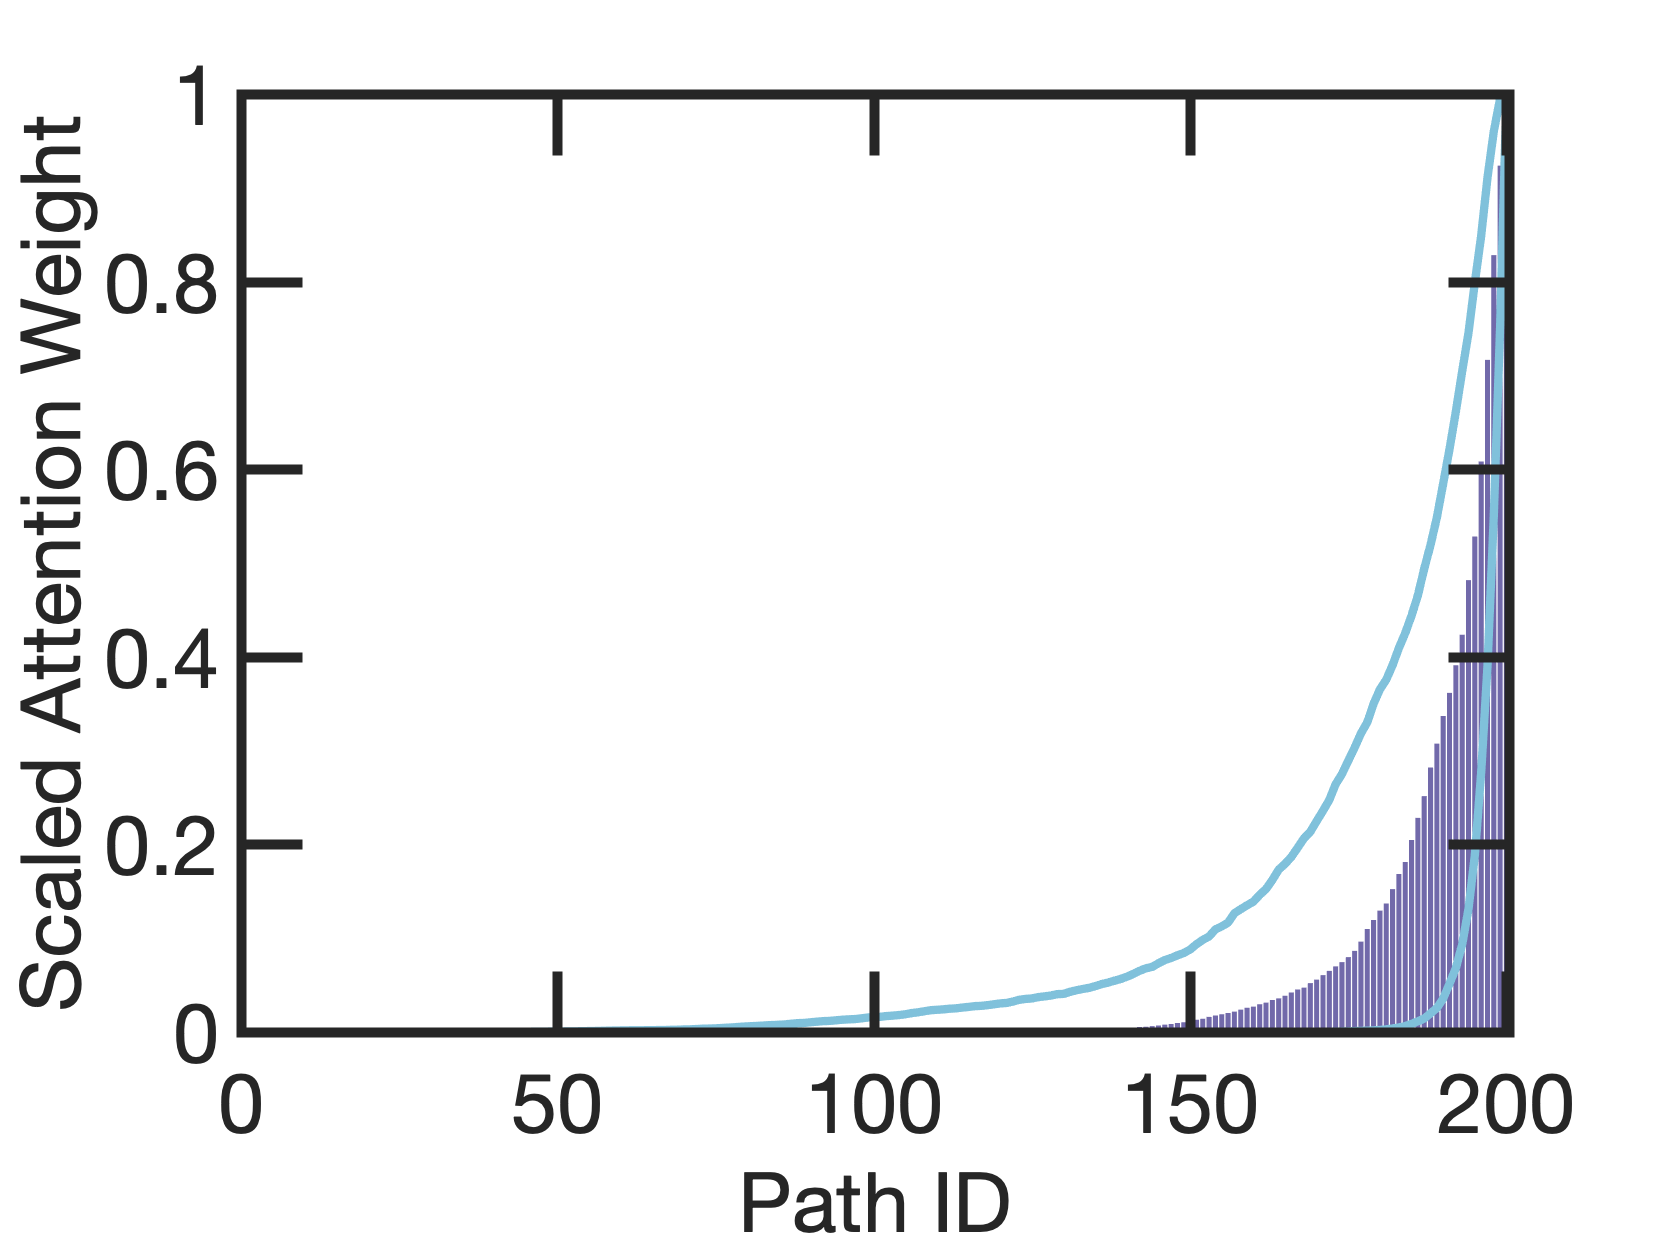
\includegraphics[width=\textwidth]{path_also_see_test.png}
    \caption{\scalebox{0.9}{$also\_see$}}
    \label{fig:path_weights_1}
  \end{subfigure}
  %
  \begin{subfigure}[b]{0.24\textwidth}
    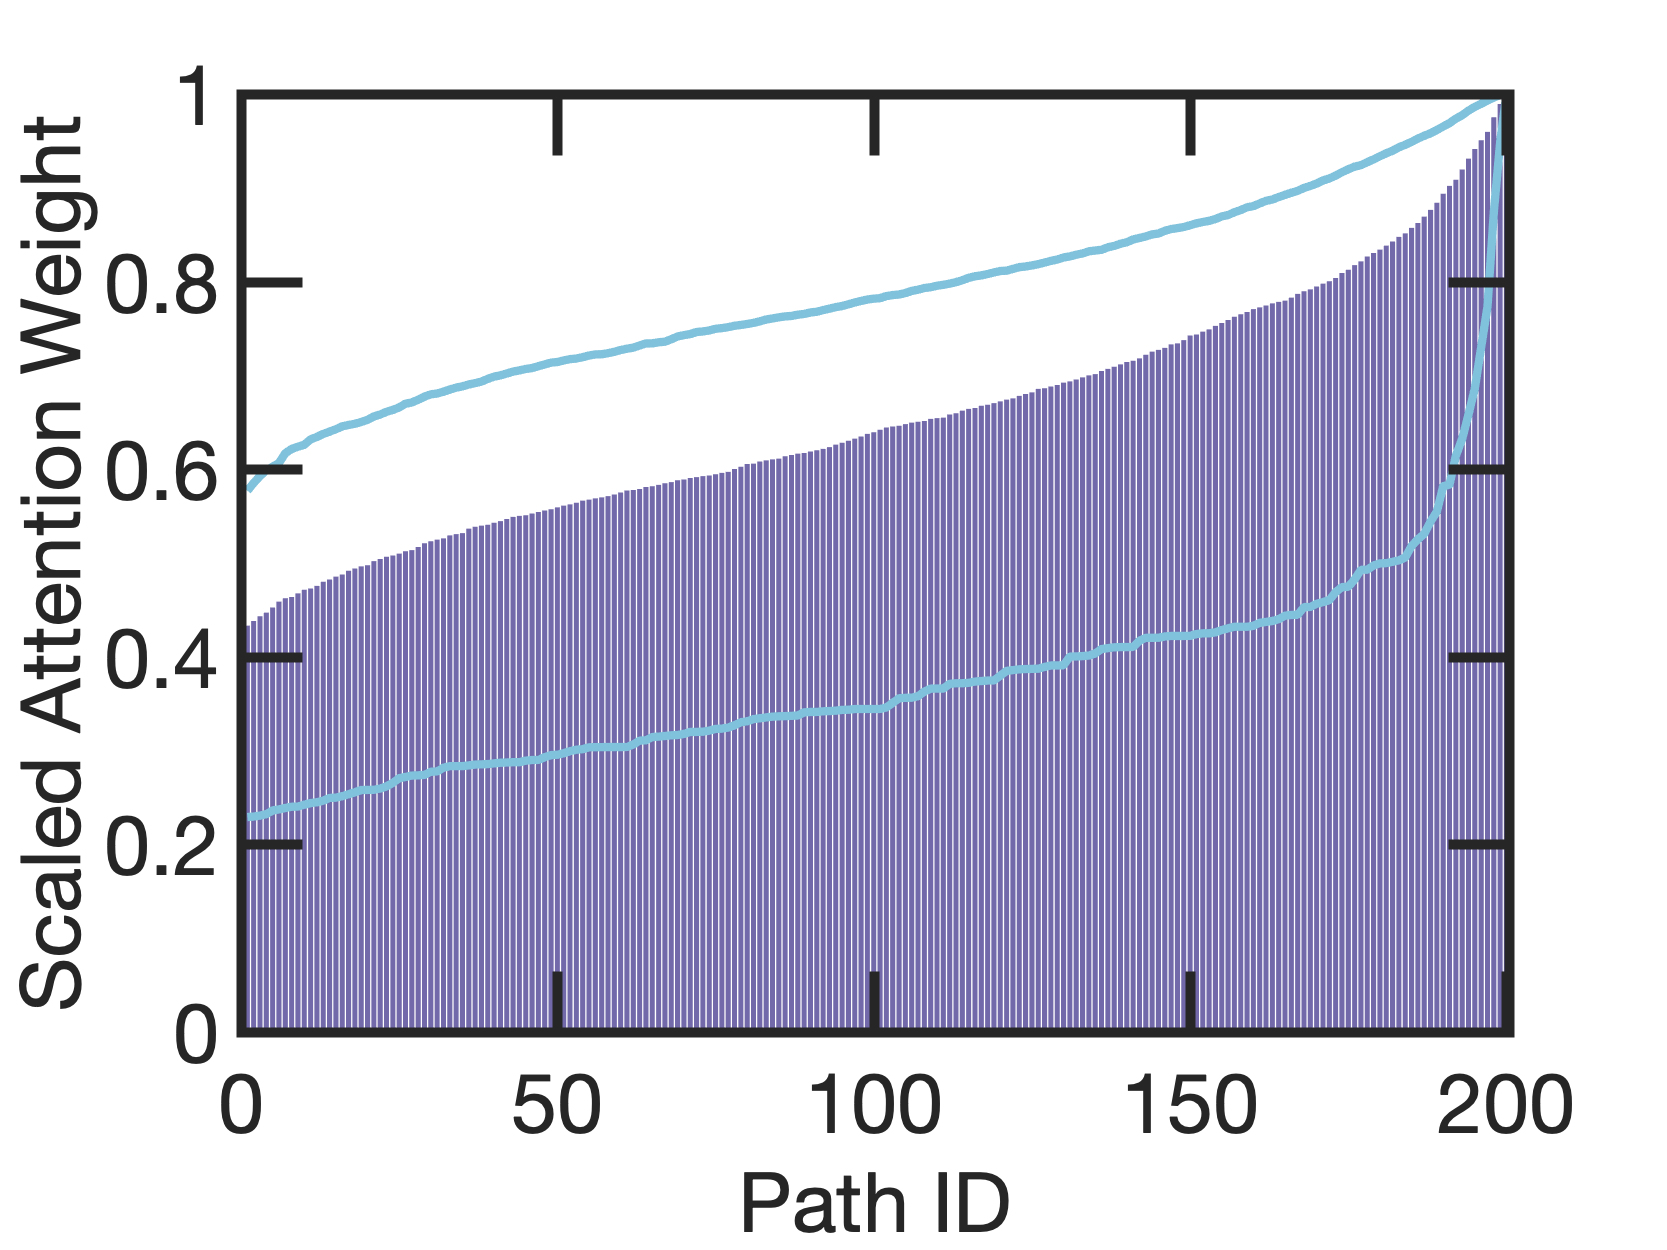
\includegraphics[width=\textwidth]{path_verb_group_test.png}
    \caption{\scalebox{0.9}{$verb\_group$}}
    \label{fig:path_weights_2}
  \end{subfigure}
  %
  \begin{subfigure}[b]{0.24\textwidth}
    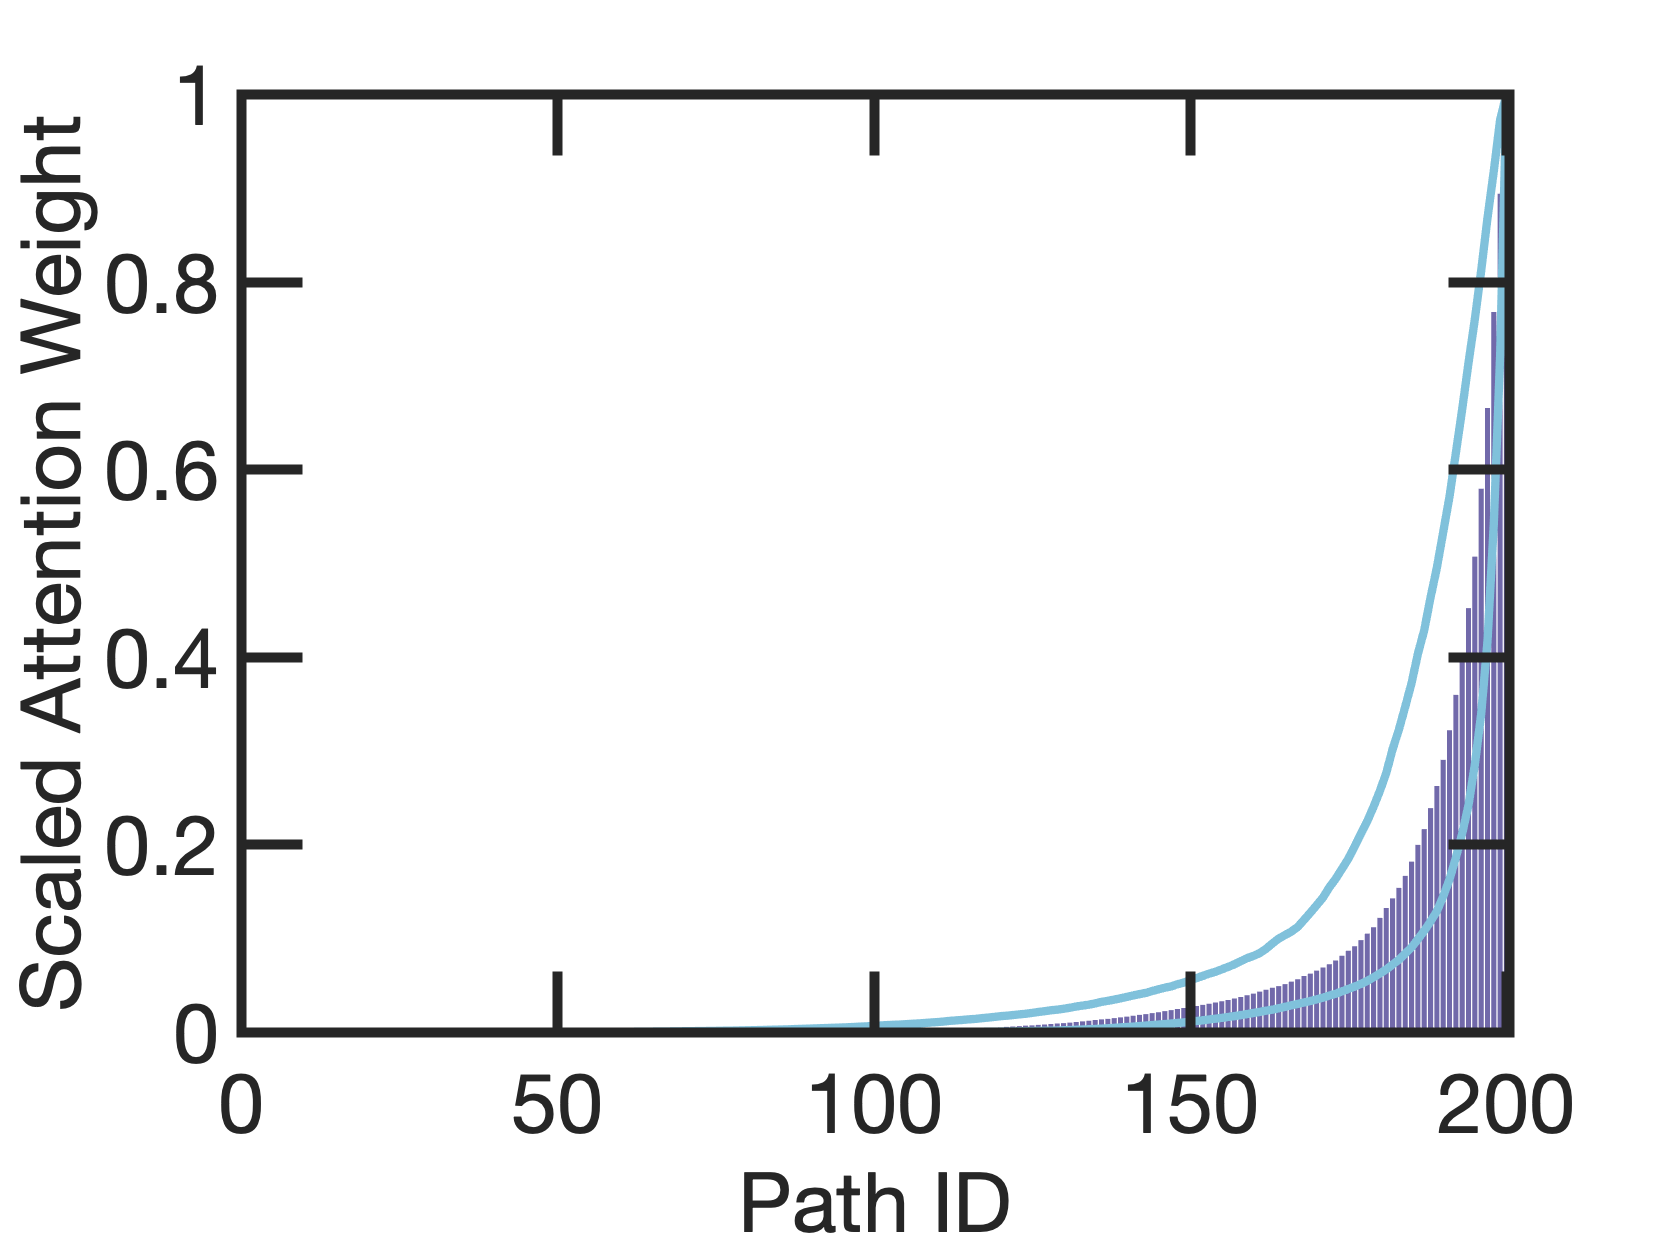
\includegraphics[width=\textwidth]{path_fb1.png}
    \caption{\scalebox{0.9}{$music/record\_label/artist$}}
    \label{fig:path_weights_3}
  \end{subfigure}
  %
  \begin{subfigure}[b]{0.24\textwidth}
    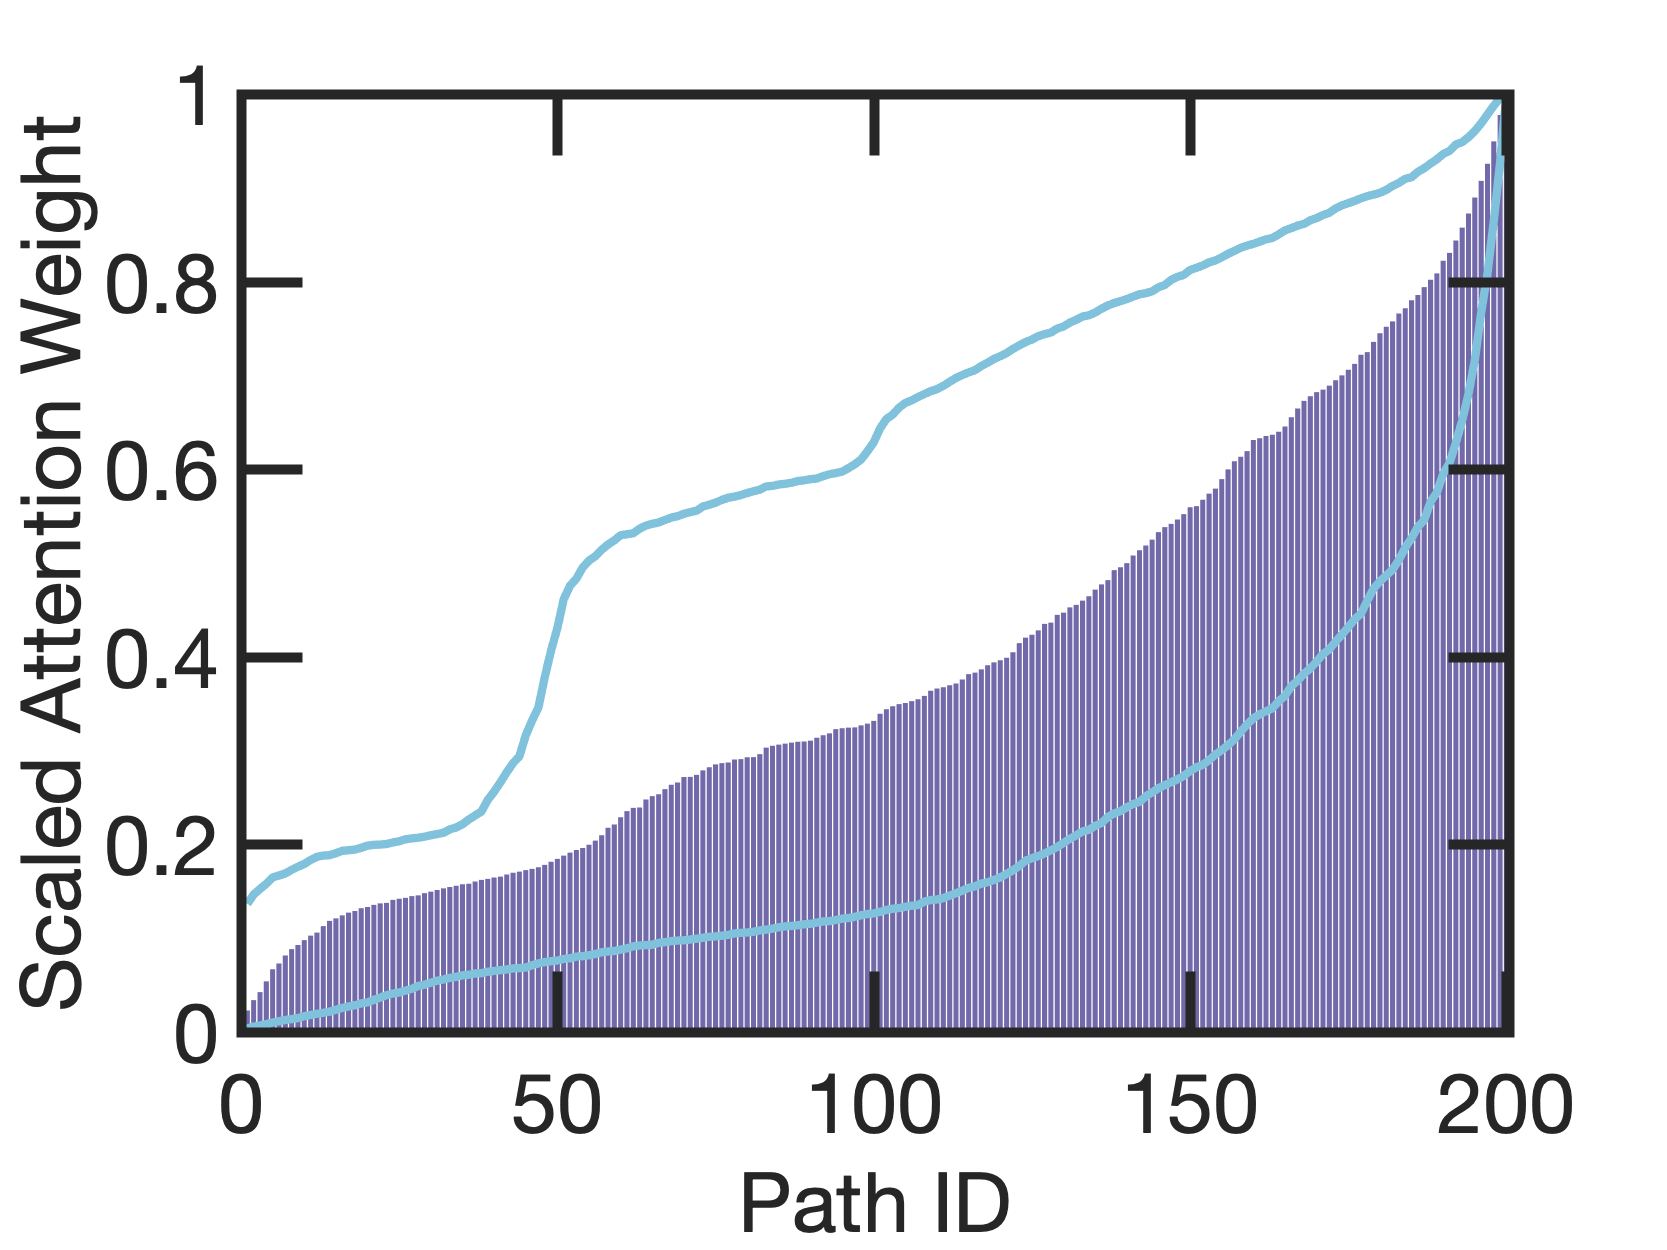
\includegraphics[width=\textwidth]{path_fb2.png}
    \caption{\scalebox{0.9}{$sports/sports\_team\_roster$}}
    \label{fig:path_weights_4}
  \end{subfigure}
  \caption{Visualization of path weight for four relations. To generate the visualization, for each relation instance, the path weights are first sorted in ascending order and normalized. Due to the varying numbers of paths between entity pairs, path weights for each relation instance are then interpolated to 200 data points. Median, 25 percentile, and 75 percentile of path weights across relation instances of each relation are plotted. }
  \label{fig:path_weights}
\end{figure*}

To extract paths between entities, we first constructed graphs from true triples in the datasets. We augmented the graphs with reverse relations following existing methods \cite{pra}. We extracted paths using bi-directional BFS. We set the maximum length of paths to 6 for WN18RR and 4 for more the densely connected FB15k-237. We randomly sampled 200 paths for each pair if there were more paths. Limiting the length of paths and sub-sampling paths are both due to computational concerns.

To create type hierarchies, we extracted inherited hypernyms available in WordNet \cite{wordnet} for WN18RR entities and used type data released in \cite{fb_types} for FB15K-237 entities. The number of type levels was automatically determined by the number of inherited hypernyms for each entity in WN18RR and the number of types for each entity in FB15K-237. We further ordered Freebase types based on their frequency of occurrence because types for Freebase entities are not strictly hierarchical. We then followed \cite{chains} to select up to 7 most frequently occurring types for each entity. As more specific types apply to fewer entities and therefore appear in fewer entities types, ordering types by frequencies allowed us to construct hierarchies of types with specific types generally in the bottom levels and abstract types generally in the top levels. Finally, for WN18RR, we mapped types to their vector representations using a pre-trained Google News word2vec model. Because we did not find a suitable pre-trained embedding for types of FB15K-237 entities, we trained an embedding with the whole model end-to-end. 

\subsection{Baselines}
We compared the performance of APR to the following  methods\footnote{The first two methods are tested with code released by \citeauthor{sfe}, and the other three with code by \citeauthor{chains}. All baselines have been tuned on the validation data and the result from the best hyperparameters is reported for each model.}\footnote{The first two baselines implement path extraction themselves, other methods and our models use the paths we extracted.}: \textit{\textbf{PRA}} from \cite{pra}, \textit{\textbf{SFE}} from \cite{sfe}, \textit{\textbf{Path-RNN\textsuperscript{A}}} from \cite{cvsm}, and the two models \textit{\textbf{Path-RNN\textsuperscript{B}}} and \textit{\textbf{Path-RNN\textsuperscript{C}}} from \cite{chains}. \textit{\textbf{Path-RNN\textsuperscript{B}}} and \textit{\textbf{Path-RNN\textsuperscript{C}}} are different in the data types they use, as shown in Table \ref{tab:results}.

% \subsection{Baselines}
% We compared the performance of APR to the following prior methods\footnote{The first two baselines implement path extraction themselves, other methods and our models use the paths we extracted.}:

% \begin{flushitemize}
    
% \item \textit{\textbf{PRA}} from \cite{pra} (see earlier description).

% \item \textit{\textbf{SFE}} from \cite{sfe} (see earlier description).

% \item \textit{\textbf{Path-RNN\textsuperscript{A}}} from \cite{cvsm}, which uses an RNN to encode relations sequentially to create vector representations of paths, which are then used for prediction. 

% \item \textit{\textbf{Path-RNN\textsuperscript{B}}} from \cite{chains}, which uses an RNN to encode concatenated vector representations of entity types and relations. 

% \item \textit{\textbf{Path-RNN\textsuperscript{C}}} from \cite{chains}, which uses an RNN to encode concatenated vector representations of entities, relations, and entity types. 
% \end{flushitemize}

\section{Results}
In this section, we report results comparing performance to the above prior methods, as well as independent validation of attention-based pooling.  We additionally present insights into the APR model and its modeling of abstraction.

\subsection{Comparison to Existing Methods}
We compared the performance of APR, paired with various pooling methods, against the baselines; Table \ref{tab:results} summarizes the results. All \textit{\textbf{APR}} variants outperformed the prior state of the art on both datasets. Directly comparing all methods that utilize LogSumExp pooling (\textit{\textbf{APR\textsuperscript{C}}} and all three \textit{\textbf{Path-RNN}} models), our results show statistically significant\footnote{As determined by a paired t-test, with each relation treated as paired data. ($p<0.05$)} improvement of \textit{\textbf{APR\textsuperscript{C}}}.  This result indicates that adding types, with the right balance between being generalizable and discriminative, helps create path patterns that allow for more accurate prediction. Our best model \textit{\textbf{APR\textsuperscript{D}}}, which further leverages attention pooling to reason about the rich contextual information in paths, is able to improve state-of-the-art performance by $26\%$ on WN18RR and $10\%$ on FB15k-237 with~($p<0.005$).

One surprising result is that \textit{\textbf{Path-RNN\textsuperscript{B}}} and \textit{\textbf{Path-RNN\textsuperscript{C}}}, even using entity and type information, still perform worse than \textit{\textbf{Path-RNN\textsuperscript{A}}} on WN18RR. We suspect that the extremely large number of entities and types in WN18RR, and the simple feature aggregation method used by these models, cause learning to not generalize even for highly adaptable neural network models. The use of abstraction helps our model generalize information from individual entities and types, and achieve more robust prediction.
%
% % Table for showing path consistency and completeness
% \begin{table*}[t]
% \centering
% \begin{tabular}{llrrrrr}  
% \toprule
% & & Train $d$  & Test $d$ & $g$ & \# Tr Path Types & \# Ts Path Types \\
% \midrule
% WN18RR & Abstract   & 0.17 & 0.19 & 0.68 & 38658 & 19503\\
%  & Specific      & 0.22 & 0.23 & 0.07 & 425099 & 136215\\
% &Attention      & 0.21 & 0.23 & 0.14 & 357662 & 119484 \\
% \midrule
% FB15k-237 & Abstract   & 0.11 & 0.12 & 0.90 &  4196 & 2894\\
%  & Specific      & 0.18 & 0.19 & 0.39 & 90189 & 42448 \\
% &Attention      & 0.17 & 0.18 & 0.31 & 54800 & 27083  \\
% \bottomrule
% \end{tabular}
% \caption{Discriminativeness $d$ and generalizability $g$ of paths along with statistics of paths.}
% \label{tab:path_quality}
% \end{table*}
%
\subsection{Pooling Methods}
We compared our proposed attention pooling to three existing pooling methods. As shown in Table \ref{tab:results}, \textit{\textbf{APR\textsuperscript{D}}} with attention pooling performs the best on both datasets. The superior performance is likely due to the pooling method's ability to collectively reason about the rich contextual information in paths. The other three methods lose information when they compress path representations to single values. 

To gain insight about the behavior of attention pooling, we visualized the path weights $\alpha_{i}$'s computed by the attention module. Figure \ref{fig:path_weights} shows visualizations of four representative relations from the two datasets. Figure \ref{fig:path_weights_1} and Figure \ref{fig:path_weights_3} show that for some relations, attention pooling focuses on small numbers of highly predictive paths. In other cases, as in Figures \ref{fig:path_weights_2} and \ref{fig:path_weights_4}, attention pooling incorporates data across a broad collection of paths. This ability to dynamically adjust attention based on context highlights the adaptability of attention pooling. %and its ability to balance generalization and discriminativeness.

%
%The performance of the other two methods also depends on the data: \textit{\textbf{Attention (LogSumExp pooling)}} performs better than \textit{\textbf{Attention (Average pooling)}} on WN18RR while the reverse is true on FB15k-237. One possible justification is the quality of paths are different for WN18RR and Fb15k-237 (we dicuss this more closely in the later section). LogSumExp pooling perform well if the small number of highly predictive paths it concentrates on during training also appear in testing data. Average pooling is more robust to unseen paths because it relies less on any single path. Our method is able to adapt to different situations by reasoning about the relative importance of paths based on the information encoded in the paths and the context of the task. 
%
%\begin{figure}[t]
%  \includegraphics[width=\linewidth]{training_curves.png}
%  \centering
%  \caption{Progress of training and testing accuracies when using the most abstract types, the most specific types, and using attention to learn the appropriate types.}
%  \label{fig:training_curve}
%\end{figure}
%
%\begin{figure}[t]
%  \includegraphics[width=\linewidth]{wn_box.png}
%  \centering
%  \caption{Distribution of training accuracies for all tested relations in WN18RR when using the most abstract type, the most specific type, and using attention to learn the appropriate type.}
%  \label{fig:wn_box}
%\end{figure}
%
%\begin{figure}[t]
%  \includegraphics[width=\linewidth]{fb_box.png}
%  \centering
%  \caption{Distribution of training accuracies for all tested relations in FB15k-237 when using the most abstract type, the most specific type, and using attention to learn the appropriate type.}
%  \label{fig:fb_box}
%\end{figure}
%

% Table for showing the effect of attention
\begin{table}[t]
\centering
\begin{tabular}{lcc}  
\toprule
& WN18RR & FB15k-237 \\
\midrule
Abstract   & 81.17 &  49.71  \\
Specific      & 82.66  &  54.55 \\
Attention (APR\textsuperscript{D}) & \textbf{84.91} & \textbf{57.35} \\
\bottomrule
\end{tabular}
\caption{MAP\% of three models using different levels of abstraction for entities.}
\label{tab:attention_effect}
\end{table}

\subsection{Correct Level of Abstraction}

% Table for qualitative results
\begin{table*}[h]
\centering
% resize
\resizebox{\textwidth}{!}{%
\begin{tabular}{lccccccc}  
\toprule
\multicolumn{8}{l}{Query Relation: has\_profession}\\
\multicolumn{8}{l}{Interpretation: Actors graduated from the same school are likely to share the same profession.}\\
&&&&&&&\\
True:&$\overset{\scalebox{1}{[Actor]}}{\text{John
Rhys-Davis}}$&$\xleftarrow{\scalebox{1}{has\_graduates}}$&$\overset{\scalebox{1}{[Thing]}}{\text{RADA}}$&$\xrightarrow{\scalebox{1}{has\_graduates}}$&$\overset{\scalebox{1}{\textbf{[Actor]}}}{\text{Micheal Gambon}}$&$\xrightarrow{\scalebox{1}{has\_profession}}$&$\overset{\scalebox{1}{[Thing]}}{\text{Actor}}$\\
False:&$\overset{\scalebox{1}{[Actor]}}{\text{Peter Ustinov}}$&$\xleftarrow{\scalebox{1}{has\_graduates}}$& $\overset{\scalebox{1}{[Thing]}}{\text{Westminster School}}$&$\xrightarrow{\scalebox{1}{has\_graduates}}$&$\overset{\scalebox{1}{\textbf{[Author]}}}{\text{Christopher Wren}}$&$\xrightarrow{\scalebox{1}{has\_profession}}$&$\overset{\scalebox{1}{[Thing]}}{\text{Scientist}}$\\
\midrule
\multicolumn{8}{l}{Query Relation: has\_genre}\\
\multicolumn{8}{l}{Interpretation: Films focusing on the same subject are likely to share the same genre. However, films depicting the same profession can have different genres.}\\
&&&&&&&\\
True:&$\overset{\scalebox{1}{[Topic]}}{\text{Life Is Beautiful}}$&$\xleftarrow{\scalebox{1}{has\_film}}$&$\overset{\scalebox{1}{\textbf{[Subject]}}}{\text{World War 2}}$&$\xrightarrow{\scalebox{1}{has\_film}}$&$\overset{\scalebox{1}{[Topic]}}{\text{Valkyrie}}$&$\xrightarrow{\scalebox{1}{has\_genre}}$&$\overset{\scalebox{1}{[Genre]}}{\text{War Film}}$\\
False:&$\overset{\scalebox{1}{[Topic]}}{\text{Air Force One}}$&$\xleftarrow{\scalebox{1}{has\_film}}$&$\overset{\scalebox{1}{\textbf{[Profession]}}}{\text{Aviation}}$&$\xrightarrow{\scalebox{1}{has\_film}}$&$\overset{\scalebox{1}{[Topic]}}{\text{Team America}}$&$\xrightarrow{\scalebox{1}{has\_genre}}$&$\overset{\scalebox{1}{[Genre]}}{\text{Political Satire}}$\\
\midrule
\multicolumn{8}{l}{Query Relation: nominee\_work}\\
\multicolumn{8}{l}{Interpretation: The best actors are likely to perform great in all movies. The same company may not always produce award winning works.}\\
&&&&&&&\\
True:&$\overset{\scalebox{1}{\textbf{[Thing]}}}{\text{Academy Actor}}$&$\xrightarrow{\scalebox{1}{nominee\_work}}$&$\overset{\scalebox{1}{\textbf{[Award Topic]}}}{\text{Network}}$&$\xleftarrow{\scalebox{1}{nominated\_for}}$&$\overset{\scalebox{1}{\textbf{[Actor]}}}{\text{Sidney Lumet}}$&$\xrightarrow{\scalebox{1}{nominated\_for}}$&$\overset{\scalebox{1}{\textbf{[Award Item]}}}{\text{Orient Exp}}$\\
False:&$\overset{\scalebox{1}{\textbf{[Award Category]}}}{\text{Emmy Comedy}}$&$\xrightarrow{\scalebox{1}{nominee\_work}}$&$\overset{\scalebox{1}{\textbf{[Tv Program]}}}{\text{Entourage}}$&$\xleftarrow{\scalebox{1}{nominated\_for}}$&$\overset{\scalebox{1}{\textbf{[Employer]}}}{\text{HBO}}$&$\xrightarrow{\scalebox{1}{nominated\_for}}$&$\overset{\scalebox{1}{\textbf{[Tv Program]}}}{\text{Gia}}$\\
\bottomrule
\end{tabular}}
% end resize
\caption{Correctly predicted examples by the proposed model on test data of FB15k-237. Despite the fact that each pair of true and false examples share the same sequence of relations, the uses of entity types at the right level of abstraction (shown in bold) help distinguish between them. Abbreviated entity and relation names are shown for clarity.}
\label{tab:qualitative_result}
\end{table*}

We further investigated whether our model learns the proposed path patterns that balance between discrimination and generalization. For comparison, we modified the best model \textit{\textbf{APR\textsuperscript{D}}} by fixing the selection of types to either the most specific level or the most abstract level. Table \ref{tab:attention_effect} shows the effect of different levels of abstraction on performance. Using a fixed level of abstraction leads to worse performance compared to using attention. This result not only confirms that balancing between generalization and discrimination makes prediction more accurate, but also that our proposed model achieves this balance by learning the correct levels of abstraction for entities.

\begin{figure}[t]
  \centering
  \begin{subfigure}[b]{0.23\textwidth}
    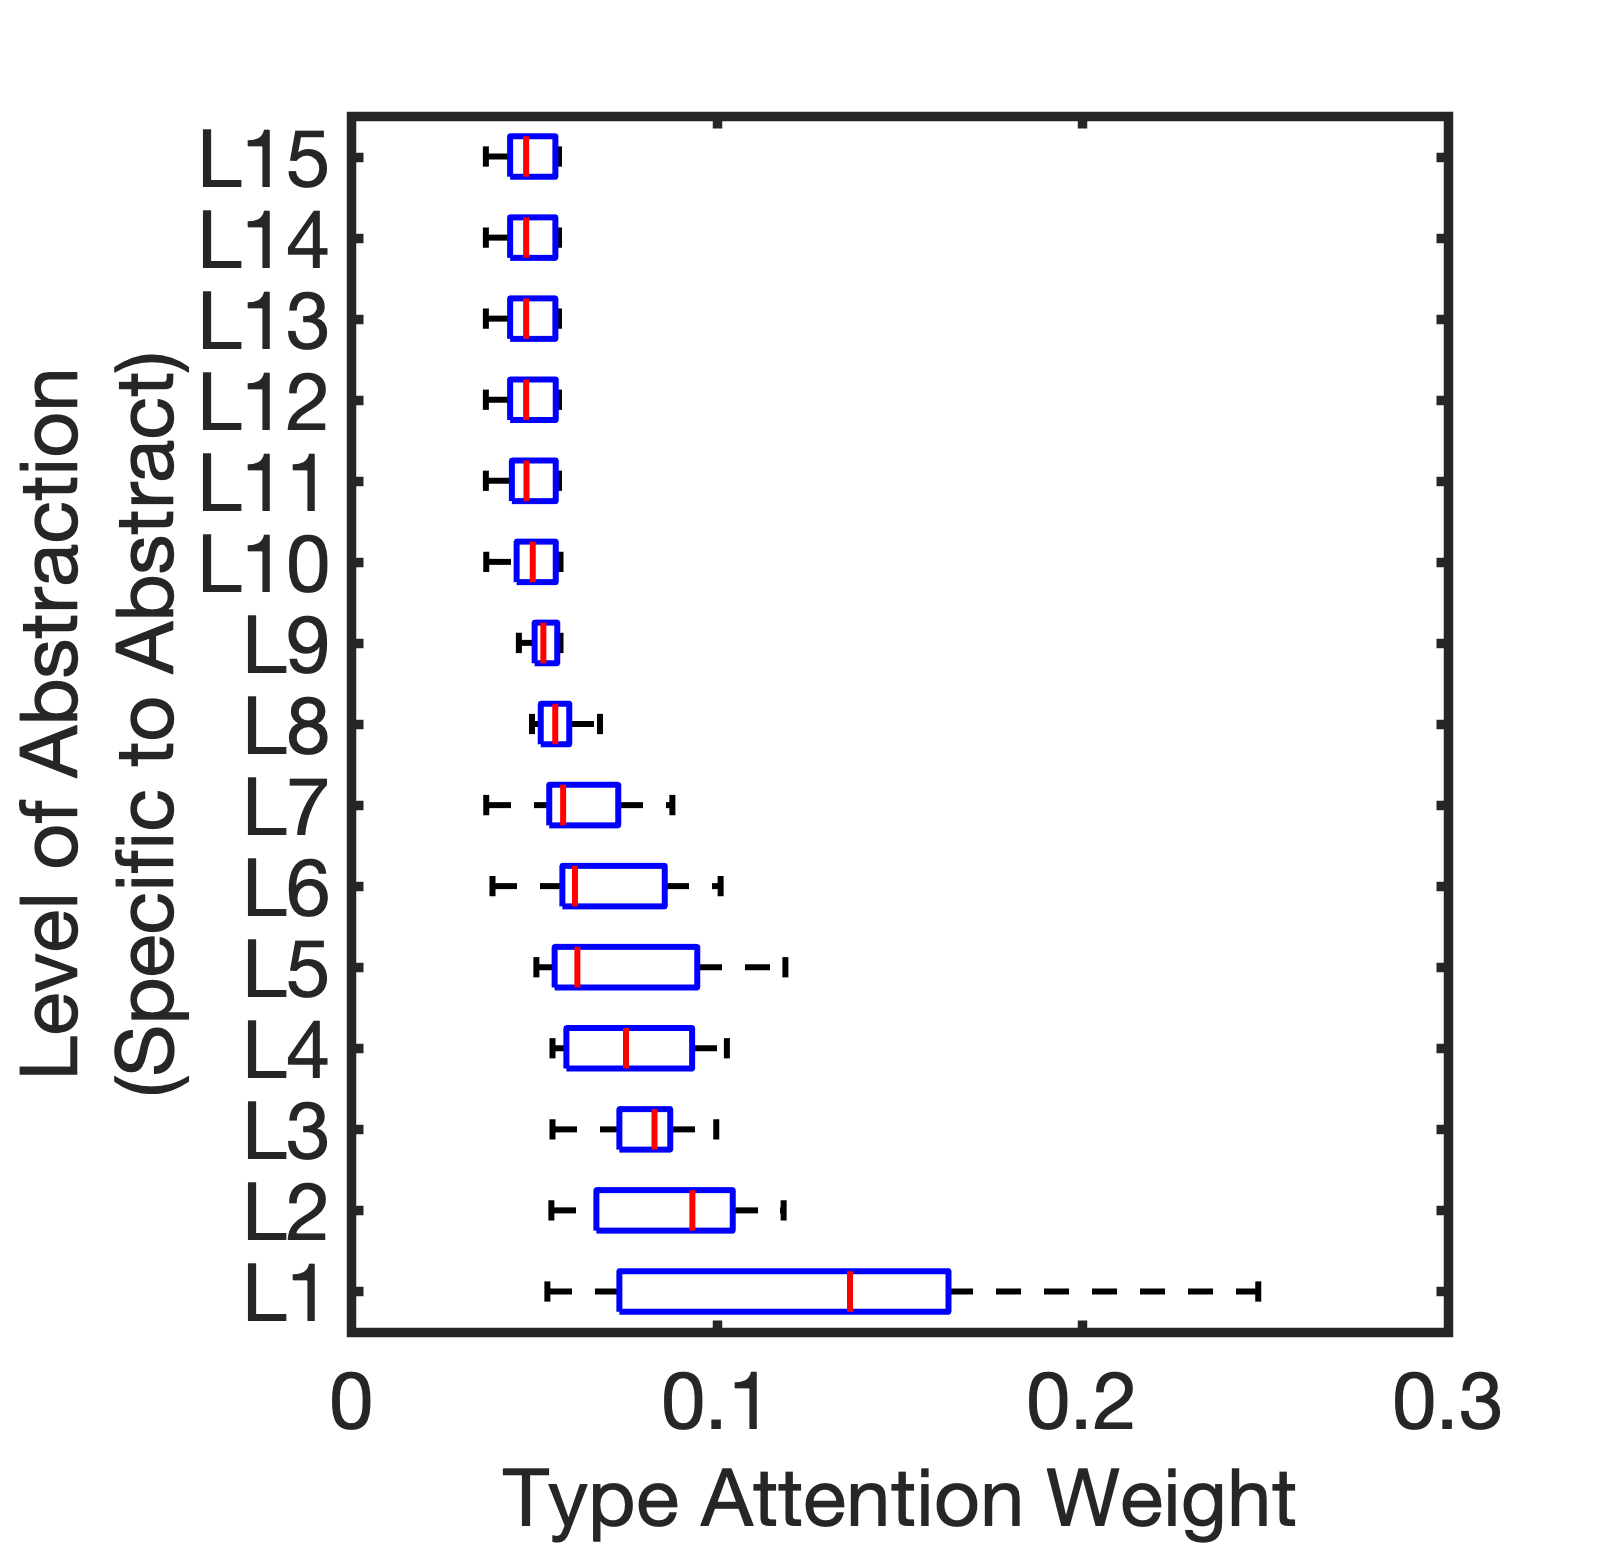
\includegraphics[width=\textwidth]{type_wn.png}
    \caption{Average type weights of WN18RR}
    \label{fig:type_weights_wn}
  \end{subfigure}
  %
  \begin{subfigure}[b]{0.23\textwidth}
    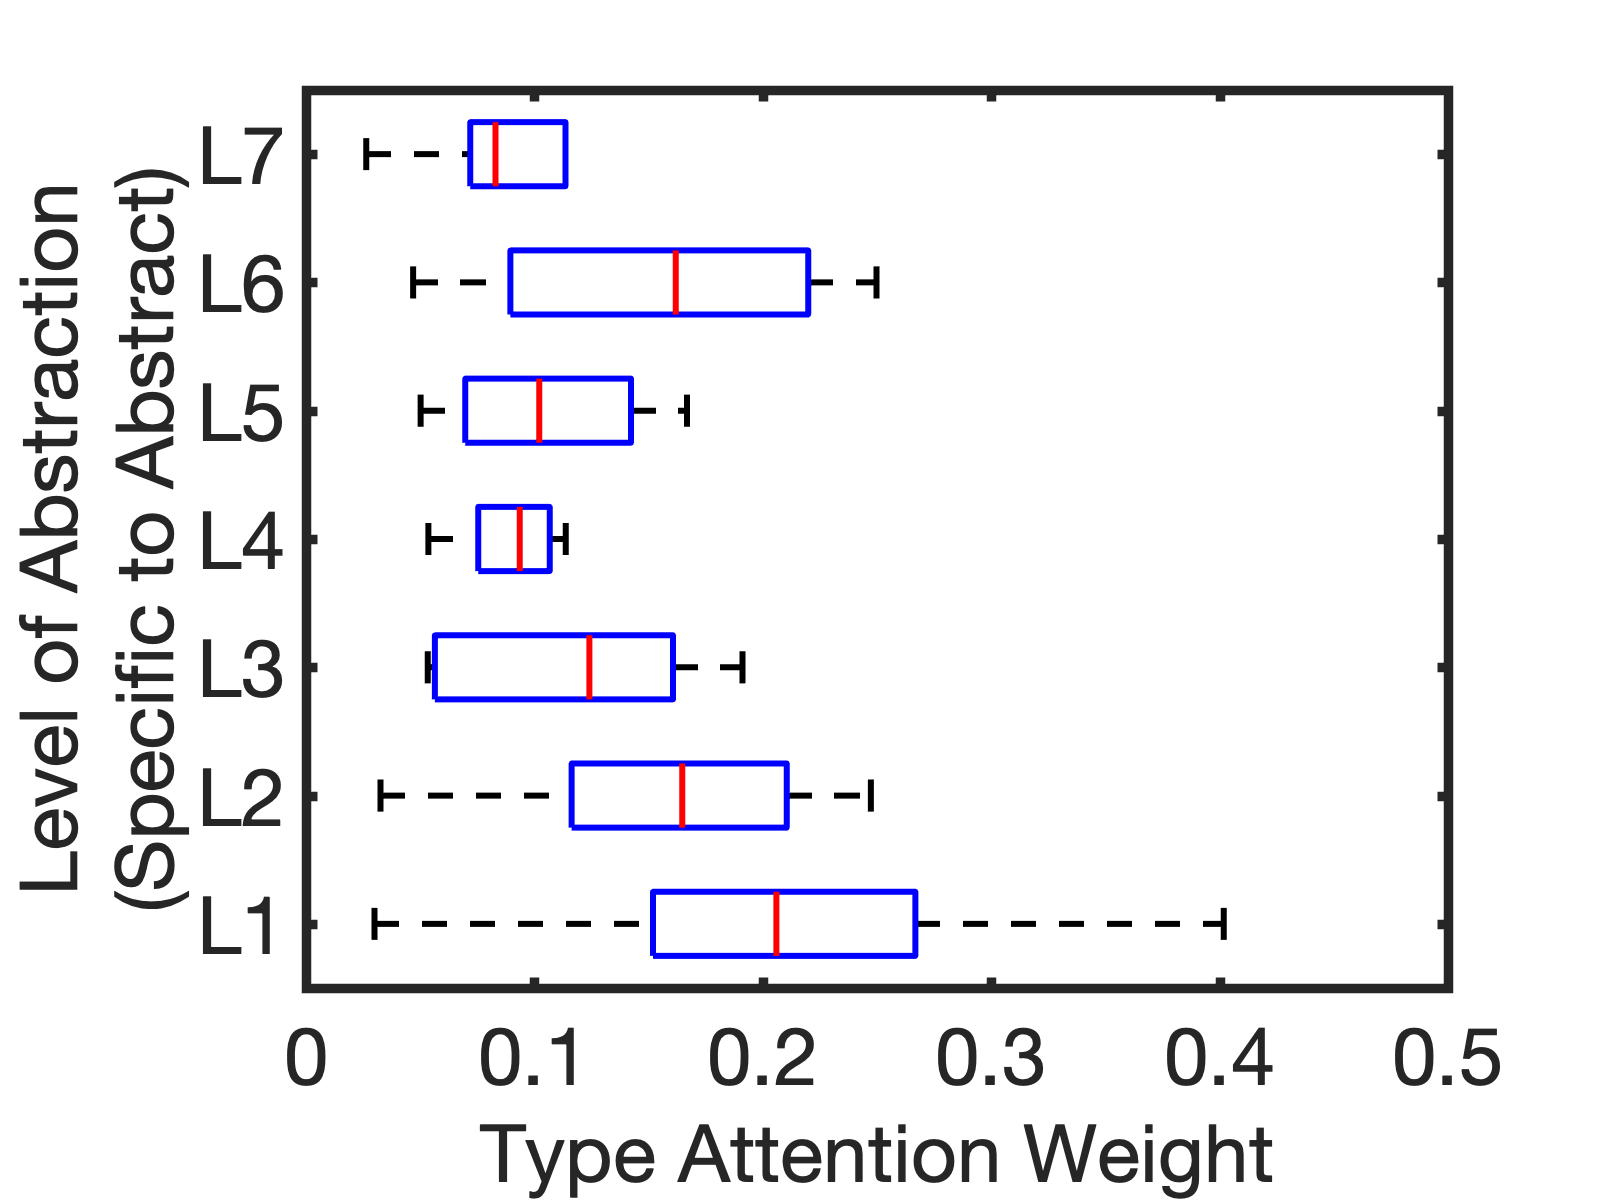
\includegraphics[width=\textwidth]{type_fb.png}
    \caption{Average type weights of FB15k-237}
    \label{fig:type_weights_fb}
  \end{subfigure}
  \caption{Box plot of average attention weights at each level. For each relation, the average attention weight of each level is computed by averaging over the weights predicted by the model at this level for all entities in all paths.}
  \label{fig:type_weights}
\end{figure}

We also examined the distribution of attention weight at different levels of type hierarchies. Figure \ref{fig:type_weights} shows that the model leveraged all levels for representing various entities. More specifically, level 1, 2, and 3 are most commonly emphasized for entities in WN18RR; level 1,2, and 6 are most often used for entities in FB15k-237. The emphasis on lower levels is expected since using the most specific level is more beneficial than using the most abstract level with evidence in Table \ref{tab:attention_effect}. However, the diversity of levels used by the model proves that not all entities should use the most specific level: different entities require different levels of abstraction.

Finally, we visualized examples of paths from prediction along with the top weighted types the model selected for entities. In Table \ref{tab:qualitative_result}, we are able to see examples that correspond strongly with human intuition. This qualitative result again verifies that the model learns a new class of rules (path patterns) that is more specific yet still generalizable. 

% Comparison with embedding methods
\begin{table}[t]
\centering
\begin{tabular}{lcc}  
\toprule
& WN18RR & FB15k-237 \\
\midrule
TuckER   & 38.16 &  40.12  \\
ComplEx-N3     & 40.89  &  40.35 \\
APR\textsuperscript{D}      & \textbf{84.91} & \textbf{57.35} \\
\bottomrule
\end{tabular}
\caption{MAP\% comparison to two SOTA embedding methods.}
\label{tab:comparison_with_embedding_methods}
\end{table}

\subsection{Comparison with Knowledge Graph Embedding Methods}
As a final point of comparison, we validated our best model \textit{\textbf{APR\textsuperscript{D}}} against two state-of-the-art KGE methods\footnote{We followed \cite{deeppath} to evaluate KGE methods on the fact prediction task. Test triples with the same relation are ranked.}: \textit{\textbf{TuckER}} \cite{tucker} and \textbf{\textit{ComplEx-N3}} \cite{complex}. As shown in Table \ref{tab:comparison_with_embedding_methods}, our model performs significantly better on both datasets. In fact, all neural-based path ranking methods (\textit{\textbf{APR}} and \textbf{\textit{Path-RNN}}) outperform the KGE methods. One possible reason that path ranking methods outperform KGE is that KGE methods require both the source $e_i$ and target entities $e_k$ in the missing triple $(e_i, r_j, e_k)$ to be known, thus failing to perform well when test entities are not present in the training set.  However, only $17.6039\%$ of FB15k-237's test data consists of new entities, and only $0.9412\%$ in WN18RR.  As a result, new entities do not alone account for the difference in performance.  This comparison additionally affirms the improved state-of-the-art performance in fact prediction achieved by our method. 

%One of the reasons that KGE methods perform worse is that their predictions rely heavily on the source $e_i$ and target entities $e_k$ in the missing triple $(e_i, r_j, e_k)$, and there are $17.6039\%$ new entities in the test set of FB15k-237 for this task. However, even when there are only a small amount of new entities, as WN18RR has 0.9412\% new entities in the test set, KGE still cannot achieve the same accuracy as path ranking based methods. This comparison again affirms the improvement of SOTA performance in fact prediction task achieved by our method. 

% Because our data split has $0.9412\%$ and $17.6039\%$ new entities in test sets that are not observed in train sets of WN18RR and FB15k-237 repectively, the embedding methods are not able to predict truth values for query triples with these new entities. \SC{Stating this here seems like you're saying improvement is only because of the new entities. This might be true for FB, but doesn't seem so for WN?} As illustrated in Table \ref{tab:task}, the presence of new entities does not affect path-ranking based methods. In fact, all \textit{\textbf{Path-RNN}} methods outperform SOTA embedding methods in this task. This comparison not only validates the importance of path-ranking based methods as they infer a wider range of missing information, but also reaffirms the improvement of SOTA performance in fact prediction task achieved by our method. \zk{Do you need a separate comparison to knowledge graph embedding methods? Why not just include in the main table and discuss it in that section?}

%FB15k-237 has on average $0.9412\% (\text{std}=1.0366)$ and WN18RR has $17.6039\% (\text{std}=10.0508)$ new entities in test set for all tested relations.

% To create representatives of paths used by the attention model, we extracted the type with the highest weight for each entity. Then we compared the different path patterns that are used by these three models,  which we denote as \textit{\textbf{Attention}}, \textit{\textbf{Specific}}, and \textit{\textbf{Abstract}}. To quantitatively evaluate whether paths are discriminative and generalizable, we define these two characteristics below. 

% We define that a path pattern (consisting of both relations and types in this case) is discriminative if this path pattern only appears in positive or negative examples, but not both. For each path pattern $\pi_i$, we count its number of occurrences in positive examples, denote $o_i^+$, and in negative examples, denote $o_i^-$. Then we calculate a ratio $r_i = o_i^+/(o_i^- + o_i^+)$, which implies a path pattern's distribution in positive and negative examples. Then we calculate the variance $d$ in the ratios $r_i$ for all path patterns. $d$ summarizes the discriminativeness of a set of path patterns. For example, if most path patterns appear in both positive and negative examples, $d$ will be small. 

% We define that a path pattern is generalizable if it appears both in training and testing. Quantitatively we define completeness as following: we assign path patterns that appear in training to set $\Pi_{train}$ and path types in testing to set $\Pi_{test}$. Then we calculate value $g$:%
% \begin{align}
% 	g = 1 - \dfrac{|\Pi_{test} \setminus \Pi_{train}|}{|\Pi_{test}|}
% \end{align} %
% where the nominator of the fraction calculates the number of path patterns in testing but not in training. We use $g$ to measure the generalizability of a set of path patterns.

% Table \ref{tab:path_quality} shows discriminativeness $d$ and generalizability $g$ of path patterns used by \textit{\textbf{attention}}, \textit{\textbf{specific}}, and \textit{\textbf{abstract}}. Train $d$ and Test $d$ columns show that discriminativeness $d$ is the smallest when using the most abstract types and the largest when using the most specific types for both training and testing. $g$ column shows that generalizability $g$ is the highest when using the most abstract types and the lowest when using the most specific types. Path patterns with the most specific types are too distinct making them hard to generalize. Our model learn path patterns that balance between generalizability and discriminativeness. 

%We invastigated this phenomenon by comparing the trends of training and testing accuracies with respect to the training iteration. Figure \ref{fig:training_curve} is a representative example of relation \textit{has\_part} from WN18RR dataset. The specific types provide high descrimination capabilities, therefore achieving higher training accuracies. Because abstract types provide minimal amount of additional information (e.g., the most abstract type for many tested entities in WN18RR is \textit{entity}), paths with most abstract types can be considered as paths only including relations. Because paths only including relations are highly generalizable, the model using the most abstract types has higher generalization capability. Becuase our method is able to maintain the ability to generalize while improve the ability to descriminate, our training accuracy is between the other two modifications and our testing accuracy is higher than both. 

% \section{Comparison with Knowledge Graph Embedding Methods}
% Both path ranking methods and knowledge graph embedding methods aim to infer missing information in KBs. However, these two classes of methods leverage different type of information, as a result, demanding different task setups and evaluations. Specifically, to make a prediction about a triple $(e_i, r_j, e_k)$, knowledge graph embedding methods examine whether the embedding of $e_i$, $e_k$, and $r_j$ have a particular structure that implies the existence of this triple. Simultaneously modeling entities and relations requires that the entities and the relation in a query triple have been learned (trained). Accordingly, in the task setup for knowledge graph embedding methods, all entities and relations in testing triples must appear in training triples. In order to assess the correctness of both the embedding of entities and relations, the evaluation of each query triple $(e_i, r_j, e_k)$ is to rank $e_k$ and its false substitutions $\{e_l|e_l\in \mathcal{E} \land (e_i, r_j, e_l) = false\}$ based on model predictions. As only one correct answer exist for each query, reciprocal rank and Hit@K are used. Path ranking methods focus on modeling relations and make a weaker assumption that query relations have been learned (trained). This change in emphasis results in a different task setup that no longer requires that entities in testing triples appear in training triples. The evaluation also changes from ranking each triple to ranking a set of triples with a particular relation. Specifically, for a relation $r_j$, all true and false triples in testing set with this relation are ranked based on model predictions. Average precision is instead used because consideration of the rankings of all correct answers is necessary.

% In order to quantitatively demonstrate the difference between these two class of methods, we present the performance of several knowledge graph embedding methods evaluating on the same data split as our proposed path ranking methods. This experiment highlights that path ranking methods are advantageous in this setup. Situations that knowledge graph embedding methods are more beneficial are left for future works to explore. 

\section{Conclusion}
This work addresses the problem of knowledge base completion.  We introduced Attentive Path Ranking, a novel class of generalizable path patterns leveraging type hierarchies of entities, and developed an attention-based RNN model to discover the new path patterns from data. Our approach results in statistically significant improvement over state-of-the-art path-ranking based methods and knowledge graph embedding methods on two benchmark datasets WN18RR and FB15k-237. Quantitative and qualitative analyses of the discovered path patterns provided insights into how APR achieves a balance between generalization and discrimination.

\section{ Acknowledgments}
This work is supported in part by NSF IIS 1564080, NSF GRFP DGE-1650044, and ONR N000141612835.

\bibliographystyle{aaai}
\bibliography{AAAI-LiuW.2859}

\end{document}
